\documentclass[9pt,letterpaper,subeqn]{beamer}
\setbeamertemplate{navigation symbols}{}
\setbeamertemplate{footline}{%
        \raisebox{5pt}{\makebox[\paperwidth]{\hfill\makebox[10pt]{\scriptsize\insertframenumber}}}}
\usefonttheme{serif}
\usecolortheme{seahorse}


\usepackage[english]{babel}
\selectlanguage{english}
\usepackage{bm}
\usepackage{booktabs}
\usepackage{color}
\usepackage[update,prepend]{epstopdf}
\usepackage{framed}
\usepackage{fleqn}
\usepackage{graphics}
\usepackage{hyperref}
\usepackage[utf8]{inputenc}
\usepackage{setspace}
\usepackage{textcomp}
\usepackage{wrapfig}
\usepackage{multirow}
\usepackage{caption}
\usepackage{subcaption}
\usepackage{subfloat}
\usepackage{hyperref}
\setbeamertemplate{caption}[numbered]
\usepackage{wrapfig}
\usepackage{tikz}


\definecolor{cadmiumgreen}{rgb}{0.0, 0.42, 0.24}
\usetikzlibrary{trees}
\usetikzlibrary{decorations.markings}

%================================================================================
%== TITLE, NAMES, DATE
%================================================================================
\title{Maternal Mortality and the Status of Women} 

 \author[Bhalotra et al.]{Sonia Bhalotra (Essex)
    \and Damian Clarke (Santiago) \\ \vspace{1mm}
    \and Joseph Gomes (Navarra)
    \and Atheen Venkataramani (Harvard)}


\date{October 2016}
%********************************************************************************
\begin{document}

\begin{frame}
\titlepage
\end{frame}

%********************************************************************************
%********************************************************************************
%*** Introduction
%********************************************************************************
%********************************************************************************
\section{Introduction}
%\begin{frame}[label=intro]
%\frametitle{The Long Shadow of Historical Institutions and Gender}
%Historical institutions cast long shadows which explain heterogeneities
%      in contemporary socio-economic outcomes (Acemoglu et al., 2001; Nunn and
%      Wantchekon, 2011). \vspace{3mm} \\
%\begin{itemize}
%    \setlength{\itemsep}{10pt}
%	\item History also plays a role in explaining how gender related preferences
%      are formed, with important links to women's contemporary well-being.
%	\begin{itemize}
%		\item Alesina et al.\ (2013): Plough use and the origins of gender roles 
%		\item Gay et al.\ (2013): Origins of gender roles embedded in language
%		\item Nunn (2012): Role of missionaries in female literacy in Africa
%	\end{itemize}
%  \item Here we argue (and document) that in many societies women are a low
%    public policy priority and show that this has \textbf{lethal implications}
%  \end{itemize}
%\end{frame}
%
%\begin{frame}
%  \frametitle{The Long Shadow of Historical Institutions and Gender}
%  In this paper we focus particularly on (female-specific) health outcomes:
%  \textcolor{blue}{rates of maternal mortality}.  We ask: \vspace{3mm} \\
%  \begin{enumerate}
%  \item Can the heterogeneity in current-day outcomes be traced back to deep-seated institutional structures? 
%  \item To what extent can this be addressed by pushing \emph{present-day} policy levers? 
%  \end{enumerate}
%\end{frame}


%%DD i suggest reducing the fontsize one point

\begin{frame}[label=MMRmap]
\frametitle{Maternal Mortality Ratio: Worldwide Inequality}
\begin{figure}[h!]
\centering
\includegraphics[scale= 0.4]{./figures/MMRworld.eps}
\end{figure}
\begin{itemize}
\item Public health emergency: 830 deaths \emph{per day}
\item 99\% of these deaths occur in the developing world
%Added sentence below. would prefer to add more numbers illustrating extreme variation in sentence below
\item Large decline since 2000 but (a) this is a late start and (b) massive variation in rates.
\item Nevertheless MDGs were not met.  ``Doubling down'' with the SDGs suggests
  importance of finding new ways to reduce rates of maternal death
\end{itemize}
%{\footnotesize \hyperlink{desc}{\textcolor{blue}{back}}}
\end{frame}


%%DD i brought this up. After 1st round of editing i will consider bringing more such descriptives to the Motivational start.
%%%D%%%\begin{frame}[label=CC1]
%%%D%%%\frametitle{Stylised Facts}
%%%D%%%\begin{figure}[htpb!]
%%%D%%%\centering
%%%D%%%\begin{subfigure}{.5\textwidth}
%%%D%%%  \centering
%%%D%%%  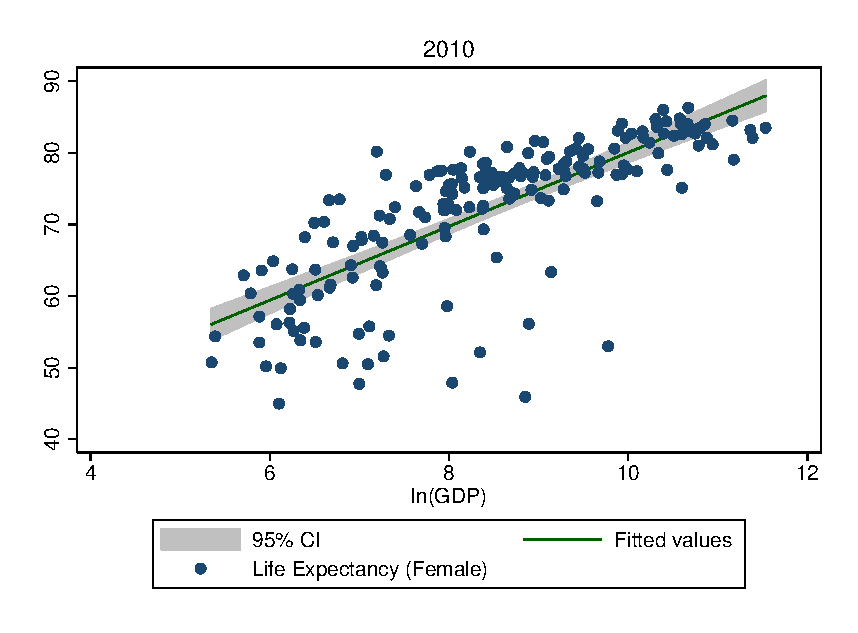
\includegraphics[scale=0.36]{./figures/lLEGDP2010.eps}
%%%D%%%  \caption{Female LE and ln(GDP)}
%%%D%%%  \label{TWINfig:fertrend}
%%%D%%%\end{subfigure}%
%%%D%%%\begin{subfigure}{.5\textwidth}
%%%D%%%  \centering
%%%D%%%  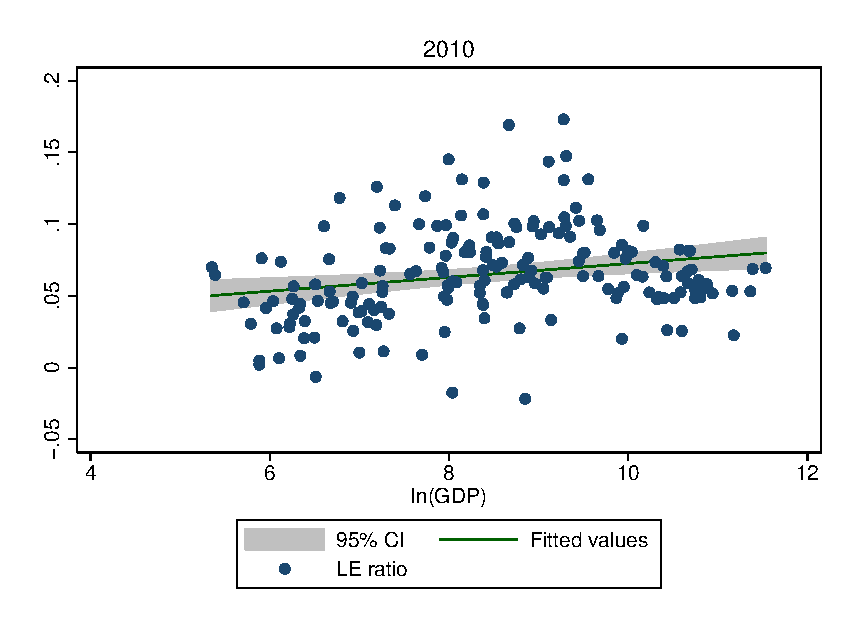
\includegraphics[scale=0.36]{./figures/lLErGDP2010.eps}
%%%D%%%  \caption{Female LE advantage and lGDP}
%%%D%%%  \label{TWINfig:eductrend}
%%%D%%%\end{subfigure}
%%%D%%%\end{figure}
%%%D%%%\begin{itemize}
%%%D%%%\item The relationship between life expectancy and GDP is clear and well-known.
%%%D%%%\item However, the relationship between the ratio of female to male life expectancy and GDP is weak.
%%%D%%%\item This suggests other factors.  We explore gendered preferences.
%%%D%%%\end{itemize}
%%%D%%%\end{frame}



\begin{frame}
\frametitle{Women's health has been a low public policy priority}
  Declines in the maternal mortality ratio (MMR) have been slower than other infectious diseases. \vspace{4mm}
\begin{itemize}
  \setlength{\itemsep}{10pt}
	\item Infant mortality decline started earlier and progressed more rapidly 
        than maternal mortality decline.
	\item Infant mortality decline has benefited from massive improvements in 
        control of infectious disease. 
	\item Historically, the same improvements led to maternal mortality declines, 
        consistent with 40-50\% of maternal deaths being the result of post-partum
        puerperal sepsis (an infection).
  \item Our hypothesis: the sluggishness of MMR decline is a function of gender 
        prejudice, (in Med/Public Health: \hyperlink{Yentl}{\textcolor{blue}
        {The Yentl Syndrome}}).
\end{itemize}
\end{frame}


%DD i have split next slide into 2. So every slide ideally makes one point and you move swiftly through them
%I have added a couple of new sentences in both of the next 2 slides
%%DD i brought this slide up so that Literature can flow into Challenge..
%%%D%%%\begin{frame}
%%%D%%%\frametitle{Maternal Mortality -- Wider Relevance}
%%%D%%%MMR impacts social and economic outcomes.  \vspace{4mm}
%%%D%%%  \begin{itemize}
%%%D%%%  \item Women's labour force participation (Albanesi and Olivetti 2009) 
%%%D%%%  \item Women's education (Alabanesi and Olivetti 2014, Jayachandran and Lleras-Muney 2008).
%%%D%%%  \item Economic growth (Lagerlof 2003, Amiri and Gerdtham 2013, Kirigia et al.\ 2006).
%%%D%%%  \item Fertility (Bhalotra and Venkataramani 2014).
%%%D%%%  \item Investments in children (Adda et al.\ 2016, Case et al.\ 2004)
%%%D%%%  \item Moreover, maternal mortality indicates more widespread maternal morbiditity.
%%%D%%%\end{itemize}
%%%D%%%\end{frame}
%%%D%%%
%%%D%%%
%%%D%%%\begin{frame}
%%%D%%%\frametitle{Related Literature}
%%%D%%%Amartya Sen, The New York Review of Books (1990) \textbf{``More Than 100 Million Women Are Missing"} (Also 1981, 2003) \vspace{4mm}
%%%D%%%\begin{itemize}
%%%D%%%%\setlength{\itemsep}{10pt}
%%%D%%%%%DD i have added refs below
%%%D%%%\item Vast literature on male-biased population sex ratios in early childhood (Miller 1981, Oster 2009, Bhalotra and Cochrane 2010, Jayachandran and Kuzeimko 2011).
%%%D%%%\item Recent work highlights that women are missing across the age (and disease) distribution (Anderson and Ray 2010, 2012).
%%%D%%%\item This work is agnostic about causes including whether prejudice in health care provision drives excess mortality amongst women.
%%%D%%%%\item We present the first attempt to focus on maternal mortality decline and assess the role of ``cultural factors'' conditional upon income (Jayachandran 2014 discusses this in more general terms).
%%%D%%%\end{itemize}
%%%D%%%\end{frame}

%DD rewriting and repositioning 
%%%D%%%\begin{frame}
%%%D%%%  \frametitle{Empirical Challenge}
%%%D%%%  \begin{itemize}
%%%D%%%  \item 
%%%D%%%  \end{itemize}
%%%D%%%\end{frame}

\frame[plain]{
\begin{center}
\textbf{Empirical Strategy}\\
\end{center}
}

%%DD i rewrote below pl check syntax
\begin{frame}
  \frametitle{Identification -- Measures of gendered preferences}
  It is difficult to define preferences over gender.  Further, it is difficult to find exogenous variation in gendered preferences. We use three complementary approaches that exploit variation in: \vspace{3mm}
  \begin{spacing}{1.3}
  \begin{enumerate}
  \item   Women's political rights. 
  \item   Stated preferences for boys over girls (in fertility).
  \item   Historical institutions that have influenced the status of women over long periods of time (pre-determined preferences).
    \begin{itemize}
    \item Linguistic structure 
    \item Historical spread of protestant vs catholic missions (sub-national)
    \end{itemize}
  \end{enumerate}
  \end{spacing}
\end{frame}


%%%D%%%%DD i added new slide below pl check syntax
%%%D%%%\begin{frame}
%%%D%%%  \frametitle{Identification -- Placebo, mechanisms}
%%%D%%%   \begin{itemize}
%%%D%%%  \item Previous research shows that women (voters and politicians) have stronger preferences over health than men (Miller 2008, Bhalotra and Clots-Figueras 2013).
%%%D%%%	\item To distinguish this from our particular focus on women's health, we use tuberculosis or pneumonia (more gender-neutral conditions) as a placebo outcome.
%%%D%%%	\item We study mechanisms by modeling antenatal care and birth attendance as a function of indicators of gendered preferences.
%%%D%%%	\item We allow the relationship to vary with economic development (GDP)
%%%D%%%\end{itemize}
%%%D%%%\end{frame}

%%DD we need a new slide here called Data. content as below-
%%%D%%%\begin{frame}
%%%D%%%  \frametitle{Data}
%%%D%%%  Measurement is a challenge. We consult data from a range of sources:
%%%D%%%  \begin{itemize}
%%%D%%%    \item MMR: annual cross-country data released in 2016 by the Maternal Mortality Estimation Inter-Agency Group (1990-2016, 181 countries)
%%%D%%%    \item MMR: annual, sub-national data created by us from DHS surveys: 60 low and middle income countries (1985-2012)
%%%D%%%    \item Political rights: American suffrage (Miller 2008), contemporary quotas (quotaproject.org), women in parliament (IPY)
%%%D%%%    \item Social, economic and more common-place political rights: Cingranelli et al.\ (2014)
%%%D%%%    \item Stated preferences for sons: DHS 1969 to 2012: 63 countries.
%%%D%%%    \item Linguistic structure: World Atlas of Language Structure (2011)
%%%D%%%    \item Protestant vs catholic missions in colonial Africa: Nunn (2012)
%%%D%%%%% anything else we use.
%%%D%%%  \end{itemize}  
%%%D%%%\end{frame}
%%%D%%%
%%%D%%%
%%%D%%%
%%%D%%%%%DD the Mechanisms are important and must be in the Intro.
%%%D%%%\begin{frame}
%%%D%%%\frametitle{Women's Political Rights}
%%%D%%%%%DD please check syntax since i added a 2nd point below (mech)
%%%D%%%Does maternal mortality decline respond to women achieving voice or decision making capacity in public policy?  \\
%%%D%%%Do women politicians allocate more resources to interventions that lower MMR (antenatal care, birth-attendance).
%%%D%%%\vspace{4.5mm}
%%%D%%%\begin{itemize}
%%%D%%%  \setlength{\itemsep}{9.5pt}
%%%D%%%	\item Womens' suffrage: Historical reform in the US interacted with medical innovation to produce state-varying MMR reductions.
%%%D%%%  \item Quotas for women in parliament: Wave of contemporary reforms since 1990.
%%%D%%%\end{itemize}
%%%D%%%\end{frame}


%********************************************************************************
%********************************************************************************
%*** Sulfa results
%********************************************************************************
%********************************************************************************
\section{Political Voice}
\frame[plain]{
\begin{center}
%\textbf{Methods and Results}\\
%\vspace{2mm}
\textbf{(1) Political Voice}\\
\end{center}
}
\subsection{Women's Suffrage- heterogeneous impacts of medical innovation for MMR}
\begin{frame}[label=USAHistory]
\frametitle{(A) Suffrage x Antibiotics for maternal infections}
\textbf{Hypothesis}: Extending the franchise to women led to more rapid MMR decline \\
\vspace{3mm}

\textbf{Method}: We cross this with a second natural experiment and estimate \hyperlink{sulfDD}{\textcolor{blue}{difference-in-differences}}.
\begin{enumerate}
\item[a)] Federal law changed in 1920 (19th amendment). But some states reformed earlier, creating variation in duration of exposure to women's influence in policymaking (Miller 2008)
\item[b)] The introduction of antibiotics (sulfonamides) in 1937 led to a 40\% decline in MMR in aggregate, but with vast state variation (Jayachandran et al. 2010, Bhalotra and Venkataramani 2013).
%%DD we must use the placebo wherever we have it
  %%DD I would prefer to display here the eq now on slide 34 in appendix (and i suggest keeping the 1st 2 sentences after the eq in small font but if you'd rather just speak them thats fine too since slides should not be too crowded.
  %%SB: I have currently left off.
\end{enumerate}
\vspace{3mm}
\textbf{Placebo}: We also show results for pneumonia which affects both genders (but boys more)%We also show results for TB decline. Since pneumonia affects both genders (but boys more), this acts as a placebo, [[[NICE POINT distinguishing women's preferences over health from women's preferences over women's health.]]]
\end{frame}


\begin{frame}[label=MMREvent,plain]
\begin{figure}
\caption{Differential impact of antibiotics in early vs late suffrage states}
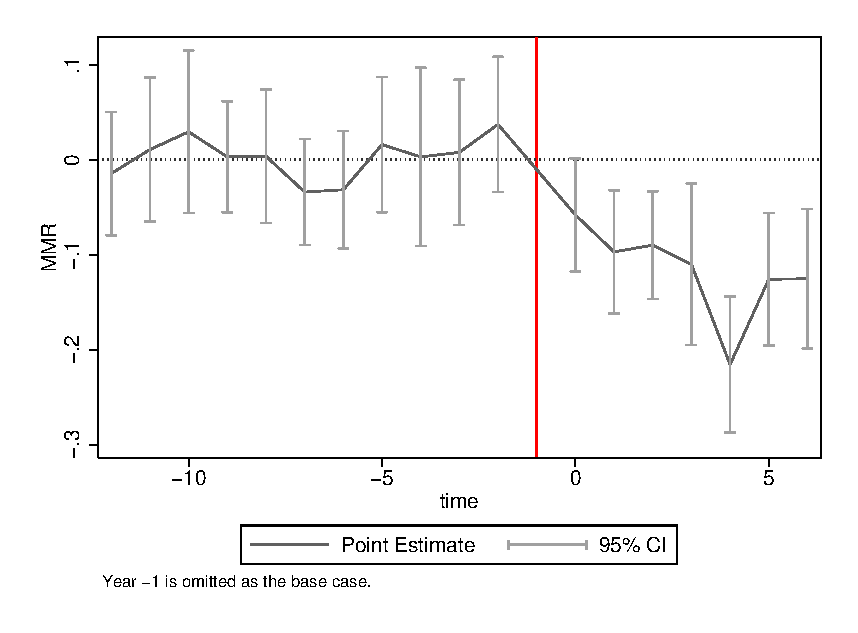
\includegraphics[scale=0.7]{./figures/eventMMR.eps}
\end{figure}
\end{frame}


%%DD add Pneumonia placebo graph here. it is on slide 40
\begin{frame}[label=IPREvent,plain]
\begin{figure}
\caption{Pneumonia (Placebo) impact of antibiotics in early vs late suffrage states}
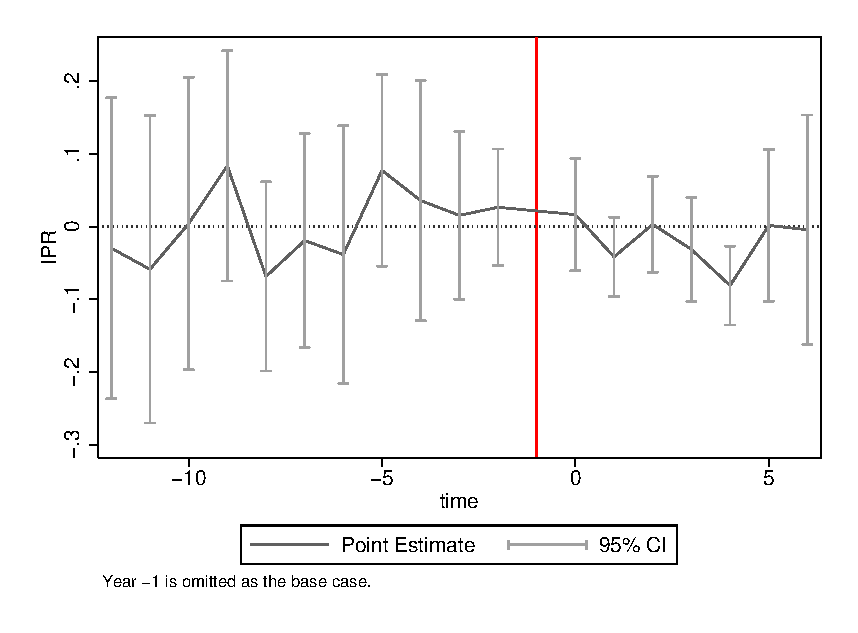
\includegraphics[scale=0.7]{./figures/eventIPR.eps}
\end{figure}
\hyperlink{DDreg}{\textcolor{blue}{regression-based estimates}}
\end{frame}

%%DD i would like to show the table on slide 39. We do show tables for other results. if you would rather not then at least add hyperlink to it above so it is an option.

%%%D%%%\begin{frame}
%%%D%%%\frametitle{(A) Suffrage x Antibiotics for maternal infections}
%%%D%%%The event study shows that MMR decline was sharper after 1937 in states in which women had political voice for longer. The effect is large: $>$10\% reduction in rates of maternal death.\\ \vspace{4mm}
%%%D%%%%%DD WE SHOULD ADD EFFECT SIZE HERE. OTHERWISE LOOKS WEAK.
%%%D%%%%XXXXDC
%%%D%%%The event study shows that this is not driven by differential pre-trends in early vs late reformers.
%%%D%%%%\vspace{3mm}
%%%D%%%%\begin{itemize}
%%%D%%%%\item No similar differential effect is seen in rates of infant pneumonia
%%%D%%%%  deaths, despite a similar large global reduction
%%%D%%%%\item This effect is sharp and large (cf 10\%) for gender-specific outcome
%%%D%%%%\end{itemize}
%%%D%%%\end{frame}


%********************************************************************************
\subsection{Quotas for  Women in Parliament}
\begin{frame}[label=Quotas]
\frametitle{(B) Quotas and Women in Parliament}
\textbf{Hypothesis}: Increasing representation of women in parliament leads to faster
reductions in MMR \\
\vspace{3mm}

\textbf{Context}: Since 1990, a number of countries have implemented quotas for women in government
 \\
\vspace{3mm}

\textbf{Method:} We use event studies to estimate both the first-stage impact of quotas on women in parliament and the reduced form impact of quotas on MMR decline. We estimate:
\begin{eqnarray}
  \log(MMR)_{ct} &=& \alpha_0 + \sum_{j=1}^J \tau_{-j}\cdot Quota_{c,t-j} + \sum_{k=1}^K \tau_{+k}\cdot Quota_{c,t+k} \nonumber \\
  && + \mu_c + \lambda_t + \varepsilon_{ct} \nonumber
\end{eqnarray}


%%DD i shortened text a lot so here we should display the event study eq on slide 46 here; it is ok to show just eq without teh text after it

\end{frame}


%%DD i would like to show our initial pic with trends in MMR, WomenParl and Quotas from the Lancet pdf here. In the quotas.pdf which included econ-results it is fig 1 and fig 5


\begin{frame}
  \frametitle{Descriptive Trends: 1990-2013}
\begin{figure}[htpb!]
  \begin{center}
    \caption{Reserved Seats, Women in Parliament and Maternal Mortality over Time}
    \label{fig:time}
    \begin{subfigure}{.5\textwidth}
      \centering
      \includegraphics[scale=0.36]{./figures/reservedSeatsWP.eps}
      \caption{Reserved Seats and Women in Parliament}
      \label{fig:seatsWP}
    \end{subfigure}%
    \begin{subfigure}{.5\textwidth}
      \centering
      \includegraphics[scale=0.36]{./figures/WomParlMMR.eps}
      \caption{Women in Parliament and Maternal Mortality}
      \label{fig:WPMMR}
    \end{subfigure}
  \end{center}
\end{figure}
\end{frame}

%%DD I THINK IMPORTANT TO ADD THE EVENT STUDY LINKING QUOTAS TO WOMEN IN PARLIAMENT HERE.it is on slide 49

\begin{frame}[label=quotaWP]
  \begin{figure}
    \caption{Event Study: Reserved Seats and Women in Parliament}
    \includegraphics[scale=0.74]{./figures/eventWomParl.eps}
  \end{figure}
\end{frame}

\begin{frame}[label=quotaMMR]
  \begin{figure}
    \caption{Event Study: Reserved Seats and ln(Maternal Mortality Ratio)}
    \includegraphics[scale=0.7]{./figures/eventlnMDeath.eps}
  \end{figure}
  %\hyperlink{quotalnMMR}{{\footnotesize Identical findings for \textcolor{blue}{Maternal Mortality Ratio}}}
\end{frame}

%%DD Slide 50 looks better than above no? Is it different?

%%DD add TB placebo graph here.

%%DD Show table of results from slide-47 here (or if you dont like this then at least a hyperlink to it)

\begin{frame}[label=quotaTabs]
  \frametitle{Reserved Seats, Women in Parliament and Maternal Mortality}
  \input{./tables/table2.tex}
\end{frame}


%%%D%%%\begin{frame}
%%%D%%%\frametitle{(B) Quotas for Women in Parliament}
%%%D%%%Reservation of a share of seats for women resulted in the expected increase in the share of women in parliament, and to faster MMR decline.
%%%D%%%%%DD WE SHOULD ADD EFFECT SIZEs HERE. OTHERWISE LOOKS WEAK.there are effect sizes on p.22 - if these are the latest and match the results we show then it is just a matter of pasting them here (and in quota results sheet)
%%%D%%%\end{frame}


%%DD i brought this up as it is quasi-political. We need to be sure if asked in seminar and need to write clearly in paper whether these are mandated rights. sounds like it from word "`rights"'
%SB: My preference for Essex would be to remove this section (to appendices) to get through everything
%%%D%%%\subsection{Women's Rights}
%%%D%%%\begin{frame}[label=WomensRights]
%%%D%%%\frametitle{Women's Rights- Political, Economic and Social}
%%%D%%%Recent compilation of country$\times$year data on women's rights (Cingranelli et al.\ 2013) \vspace{4mm}
%%%D%%%\begin{itemize}
%%%D%%%		%\item Political, Economic \& Social rights.
%%%D%%%		\item \textbf{Political Rights} - e.g. rights to vote, run for political office.
%%%D%%%		\item \textbf{Economic Rights} - e.g. equal pay for equal work, free choice of profession without the need to obtain a husband or male relative's consent, right to work at night.
%%%D%%%		\item \textbf{Social Rights} - e.g. equal inheritance, right to initiate divorce, freedom from genital mutilation or forced sterilization.
%%%D%%%\end{itemize} \vspace{4mm}
%%%D%%%%%DD pl check syntax i added stuff below
%%%D%%%Panel data identification: control for country and year fixed effects, GDP. 
%%%D%%%Standard errors clustered at country level. Test robustness to country-specific linear trends and continent$\times$year fixed effects.  We also control for democracy since this is likely to be correlated with women's rights.
%%%D%%%\end{frame}

%\item Economic rights. %equal pay for equal work; free choice of profession or employment without the need to obtain a husband or male relative's consent; gainful employment without the need to obtain a husband or male relative's consent; equality in hiring and promotion practices; job security (maternity leave, unemployment benefits, no arbitrary firing or layoffs, etc...); non-discrimination by employers; be free from sexual harassment in the workplace; work at night; work in occupations classified as dangerous; work in the military and the police force.  
		%\item Social rights.  %equal inheritance; enter into marriage on a basis of equality with men; travel abroad; obtain a passport; confer citizenship to children or a husband; initiate a divorce;  own, acquire, manage, and retain property brought into marriage; participate in social, cultural, and community activities; an education; choose a residence/domicile; freedom from female genital mutilation of children and of adults without their consent; and the freedom from forced sterilization.


%%%D%%%\begin{frame}[label=Rights]
%%%D%%%\frametitle{Women's Rights}
%%%D%%%\begin{table}[htbp]\centering
\def\sym#1{\ifmmode^{#1}\else\(^{#1}\)\fi}
\caption{MMR and Women's Rights}
\scalebox{0.6}{
\begin{tabular}{l*{6}{c}}
\toprule
                    &\multicolumn{1}{c}{(1)}   &\multicolumn{1}{c}{(2)}   &\multicolumn{1}{c}{(3)}   &\multicolumn{1}{c}{(4)}   &\multicolumn{1}{c}{(5)}   &\multicolumn{1}{c}{(6)}   \\
                    &     MMR \ \   &     MMR \ \   &     MMR \ \   &     MMR \ \   &     MMR \ \   &     MMR \ \   \\
\midrule

 \textsc{Panel A: Political Rights}&&&&&\\ 
Political Rights    &      -44.19** &       -1.79   &       -2.47   &     -367.13***&     -346.89***&     -256.74***\\
                    &     [18.54]   &     [17.54]   &     [17.30]   &     [74.73]   &     [77.60]   &     [80.30]   \\

R-squared           &        0.93   &        0.93   &        0.93   &        0.94   &        0.94   &        0.94   \\
Observations        &         757   &         757   &         757   &         757   &         757   &         757   \\

 &&&&&& \\
 \textsc{Panel B: Economic Rights}&&&&&\\ 

Economic Rights     &       11.11   &       10.79   &        6.62   &     -165.37*  &     -164.61*  &     -103.71   \\
                    &     [23.50]   &     [22.39]   &     [22.24]   &     [97.86]   &     [97.27]   &     [87.01]   \\

R-squared           &        0.92   &        0.93   &        0.93   &        0.93   &        0.94   &        0.94   \\
Observations        &         755   &         755   &         755   &         755   &         755   &         755   \\

 &&&&&& \\
 \midrule Year FE&&Y&Y&Y&Y&Y\\ Democracy controls &&&Y&&Y&Y\\ 
Rights$\times$ GDP &&&&Y&Y&Y\\ Democracy$\times$ GDP &&&&&&Y\\

 \bottomrule 
 \end{tabular}}\end{table}

%%%D%%%\hyperlink{RightsComp}{Similar findings for \textcolor{blue}{composite measures}}
%%%D%%%\end{frame}

%SB: I would prefer to talk through numbers rather than adding in a separate slide.  I am better responding to numbers in tables as we go rather than summing up, as by the time I get to the summary slide I always find that I am repeating myself.  Of course the points themselves I absolutely agree with, and agree are important.

%%DD if this is still correct here is the effect size from slide-22: to insert on a new page here but we should add the results for econ and social rights. If social rights have no impact we should say so- it seems odd that the above table displays only pol and ec but ok for slides if social is not signif and we say so.
%A 1 s.d.increase in women's political rights leads to 9 fewer maternal deaths per 100,000 live births which is 3.42% of the mean and 2.48% of the s.d. in an average GDP country
%Add effect sizes for soc and ec rights here.


%%DD in terms of titles, the quota analysis is (a) cross country and (b) contemporaneous so neither of these subtitles is right to distinguish the next slides. i am using the 3-way structure i put on a slide above.
%********************************************************************************
\section{Stated Preferences}
\frame[plain]{
\begin{center}
\textbf{(2) Stated Preferences for Sons}\\
\end{center}
}


\subsection{Desired Sex Ratio of Births}

\begin{frame}
\frametitle{Stated Preferences for Sons}
\textbf{Hypothesis}: Stronger stated preferences for son mark gendered preferences in society and influence reductions in MMR.
\vspace{3mm}
\begin{itemize}
\setlength{\itemsep}{15pt}
\item We construct individual and cohort-level indicators of son preference measured as women's reported desired number of sons relative to daughters (68 DHS countries).
%DD - be prepared to explain construction as below=
%\item The DSR in, say, 1990, is the DSR reported by all women who were 15-25 years of age in 1990, irrespective of when their responses are elicited.

%{\footnotesize \hyperlink{DSRMap}{\textcolor{blue}{See map}}}
\begin{itemize}
\item Low Son Preference countries: Dominican Republic (0.92); Haiti, Ukraine (0.94); Nicaragu%a (0.96), Colombia (0.99) 
\item Medium: Zimbabwe (1.08), Ghana (1.108), Tanzania (1.07) 
\item High: India (1.33), Nepal (1.42), Pakistan (1.59)
\end{itemize}
%%DD i removed what i thought was redundant stuff about methods below and retained the interesting figures above.
\item Panel data estimates, controlling for cohort and country fixed effects and GDP. 
\item We also control for desired fertility, a potential omitted variable when using stated son preference (Dasgupta and Bhat 1997, Jayachandran, forthcoming).
%\item \hyperlink{DSRIMR}{\textcolor{blue}{We observe}} that DSR is strongly linked to excess girl infant mortality
\end{itemize}
\end{frame}


%%%D%%%\begin{frame}[label=DSRMap]
%%%D%%%\frametitle{Distribution of Stated Preferences for Sons}
%%%D%%%  \begin{figure}[h!]
%%%D%%%\centering
%%%D%%%\caption{Desired Sex ratio From 63 DHS countries average for 1969-2012}
%%%D%%%\includegraphics[scale= 0.4]{./figures/DSR}
%%%D%%%\end{figure}
%%%D%%%%{\footnotesize \hyperlink{DSR}{\textcolor{blue}{back}}}
%%%D%%%\end{frame}

%%DD slide 53 map of DSR here - you can spend just one second on it in talk but it looks nice.

\begin{frame}[label=DSRanalysis]
\frametitle{Stated Preferences for Sons} 
\begin{table}[htbp]\centering
\def\sym#1{\ifmmode^{#1}\else\(^{#1}\)\fi}
\caption{MMR and Desired Sex Ratio (boys/girls)}
\scalebox{0.7}{
\begin{tabular}{l*{5}{c}}
\toprule
                    &\multicolumn{1}{c}{(1)}   &\multicolumn{1}{c}{(2)}   &\multicolumn{1}{c}{(3)}   &\multicolumn{1}{c}{(4)}   &\multicolumn{1}{c}{(5)}   \\
                    &     MMR \ \   &     MMR \ \   &     MMR \ \   &     MMR \ \   &     MMR \ \   \\
\midrule
Desired Sex Ratio   &       824.7** &       655.0** &       667.0** &       923.9***&      2627.7***\\
                    &     [329.4]   &     [299.3]   &     [286.5]   &     [252.9]   &     [617.9]   \\
ln(GDP)             &               &               &        40.9   &        12.4   &       318.5***\\
                    &               &               &      [48.5]   &      [49.8]   &     [119.6]   \\
Desired Sex Ratio$\times$ ln(GDP)&               &               &               &               &      -285.3***\\
                    &               &               &               &               &     [100.7]   \\
Constant            &      -476.0   &      -405.1   &      -712.6   &     -1514.3***&     -3371.0***\\
                    &     [358.9]   &     [325.8]   &     [494.2]   &     [483.9]   &     [734.5]   \\
\midrule
R-squared           &        0.09   &        0.92   &        0.92   &        0.93   &        0.93   \\
Observations        &         310   &         310   &         307   &         307   &         307   \\
 Country FE &&Y&Y&Y&Y\\ Year FE&&Y&Y&Y&Y\\ 
Desired Fertility&&&&Y&Y\\
\bottomrule\end{tabular}}\end{table}

\end{frame}

%%Show TB placebo at least once for these cross country panel regressions- so maybe here. It is on slide 66.
%for other stuff like women's rights etc we can add a hyperlink or if in a rush can leave out for essex but insert for world bank
\begin{frame}[label=placebo2]
  \frametitle{Stated Preferences for Sons and Placebo Outcome} 
\begin{table}[htbp]\centering
\def\sym#1{\ifmmode^{#1}\else\(^{#1}\)\fi}
\caption{TB and Desired Sex Ratio (boys/girls)}
\scalebox{0.7}{
\begin{tabular}{l*{5}{c}}
\toprule
                    &\multicolumn{1}{c}{(1)}   &\multicolumn{1}{c}{(2)}   &\multicolumn{1}{c}{(3)}   &\multicolumn{1}{c}{(4)}   &\multicolumn{1}{c}{(5)}   \\
                    &          TB   &          TB   &          TB   &          TB   &          TB   \\
\midrule
Desired Sex Ratio   &      -134.6   &       -98.4   &      -140.7   &      -131.9   &      -794.3   \\
                    &     [143.7]   &     [269.5]   &     [272.6]   &     [301.6]   &     [478.5]   \\
ln(GDP)             &               &               &       -54.5*  &       -55.2   &      -173.9** \\
                    &               &               &      [32.5]   &      [34.5]   &      [81.6]   \\
Desired Sex Ratio$\times$ ln(GDP)&               &               &               &               &       109.7   \\
                    &               &               &               &               &      [67.5]   \\
Constant            &       402.0** &       325.7   &       771.0*  &       739.9   &      1473.2** \\
                    &     [169.5]   &     [285.2]   &     [388.0]   &     [529.0]   &     [599.3]   \\
\midrule
R-squared           &        0.00   &        0.80   &        0.81   &        0.81   &        0.81   \\
Observations        &        1407   &        1407   &        1393   &        1393   &        1393   \\
 Country FE &&Y&Y&Y&Y\\ Year FE&&Y&Y&Y&Y\\ 
Desired Fertility&&&&Y&Y\\
\bottomrule\end{tabular}}\end{table}

%\begin{table}[htbp]\centering
%\scriptsize
%\caption{TB mortality rate and Stated Son Preference}
%\begin{tabular}{l*{5}{c}}
%\hline\hline
%            &\multicolumn{1}{c}{(1)}&\multicolumn{1}{c}{(2)}&\multicolumn{1}{c}{(3)}&\multicolumn{1}{c}{(4)}&\multicolumn{1}{c}{(5)}\\
%            %&\multicolumn{1}{c}{indep1}&\multicolumn{1}{c}{indep2}&\multicolumn{1}{c}{indep3}&\multicolumn{1}{c}{indep3b}&\multicolumn{1}{c}{indep5}\\
%\hline
%Desired Sex Ratio         &       26.32         &      -35.95         &      -43.32         &      -25.23         &      -52.34         \\
%            &     (72.30)         &     (45.99)         &     (42.58)         &     (39.33)         &     (193.8)         \\
%
%Log GDP        &                     &                     &      -3.352         &      -3.734         &      -8.376         \\
%            &                     &                     &     (7.483)         &     (7.286)         &     (34.96)         \\
%
%%Desired Fertility &                     &                     &                     &       15.64$^{*}$  &       15.61$^{*}$  \\
%%            &                     &                     &                     &     (9.046)         &     (9.008)         \\
%
%Desired Sex Ratio* Log GDP     &                     &                     &                     &                     &       4.310         \\
%            &                     &                     &                     &                     &     (30.28)         \\
%
%%\_cons      &       9.119         &       86.53$^{*}$  &       116.8         &       35.37         &       64.75         \\
%%            &     (81.80)         &     (51.62)         &     (71.46)         &     (71.69)         &     (218.7)         \\
%\hline
%\(N\)       &        1407         &        1407         &        1375         &        1375         &        1375         \\
%r2          &                     &       0.222         &       0.219         &       0.247         &       0.247         \\
%\hline
%Country FE        &                     &    Y                 &      Y               &     Y         &               Y         \\
%Year FE            &                     &    Y                 &      Y               &     Y         &             Y         \\
%Desired Fertility &                     &                     &                     &       Y&             Y\\
%\hline\hline
%\multicolumn{6}{l}{\footnotesize Standard errors in parentheses}\\
%\multicolumn{6}{l}{\footnotesize $^{*}$ \(p<0.10\), $^{**}$ \(p<0.05\), $^{***}$ \(p<0.01\)}\\
%\end{tabular}
%\end{table}
%{\footnotesize \hyperlink{placebos}{\textcolor{blue}{back}}}
\end{frame}



%%%D%%%\begin{frame}
%%%D%%%\frametitle{Stated Preferences for Sons}
%%%D%%%%\vspace{4mm}
%%%D%%%\begin{itemize}
%%%D%%%	\item A 1 s.d. increase in son preference results in 48 additional maternal deaths per 100,000 live births which is 10\% of the MMR mean and 11\% of the s.d.
%%%D%%%	\item We observe a similar significant relationship if we replace MMR with the ratio of female to male life expectancy.
%%%D%%%	\item This association is stronger in poorer countries. %DD add effect size if you have time, if not do for W Bank (and of course paper. i think Joseph did this for me in Essex but not sure if correct for updated results.
%%%D%%%	%%DD it is ok to leave for now but before WBank we should be more **systematic** in discussing the GDP heterogeneity for all cases shown in the paper.
%%%D%%%	\item These results are robust to controlling for desired fertility; the point estimates are larger.
%%%D%%%      %SB: The results below are related to my prior comment: I think I will present better with fewer slides to distract myself with, and talking about tables rather than a slide with the table and a separate slide explaining tables.
%%%D%%%		%DD these other effects should be described just after each result is shown above
%%%D%%%%	\item A 1 s.d.increase in women's political rights leads to 9 fewer maternal deaths per 100,000 live births which is 3.42\% of the mean and 2.48\% of the s.d. in an average GDP country
%%%D%%%%	\item Comparing reductions in MMR in early- and late-suffrage states following the arrival of sulfanide drugs in the USA:
%%%D%%%		
%%%D%%%%\begin{itemize}
%%%D%%%%		\item Early suffrage states in the USA reduced MMR by nearly 10 percentage points more than late suffrage states
%%%D%%%    %\vspace{4mm}
%%%D%%%	%	\item In comparative terms, this is approximately \emph{double} the effect seen in late-suffrage states
%%%D%%%%\end{itemize}
%%%D%%%		%\vspace{4mm}
%%%D%%%
%%%D%%%	%	\item A 1 s.d.\ increase in quotas leads to
%%%D%%%	%	\begin{itemize}
%%%D%%%		%\item an increase of 8.4\% of the mean and 11.33\% of the s.d.\ of women in parliament.
%%%D%%%    %\vspace{4mm}
%%%D%%%		%\item a fall of 33.6\% of the mean and 8\% of the s.d.\ of log of MMR.
%%%D%%%%\end{itemize}
%%%D%%%\end{itemize}
%%%D%%%\end{frame}


\frame[plain]{
\begin{center}
\textbf{(3) Historical Institutions}\\
\end{center}
}

\subsection{Grammatical Gender}
\begin{frame}
\frametitle{Historical Institutions- Linguistic structure}
\textbf{Hypothesis}: Long-standing institutions (language) shape attitudes to gender and can explain contemporary differences in MMR. \\
\vspace{3mm}

%%DD you may want to be prepared to give an e.g. of spanish vs english for eg; and add hyperlink here to slide 58

\textbf{Context}: Language and its grammatical emphasis on subordinate gender can
explain deep-seated gender biases
(Givati and Troiano 2012, Gay et al. 2016)\\
\vspace{3mm}

%%DD see if the following points can be itemized?
\textbf{Method}: Language is highly pre-determined. We use the majority language of a country and panel data estimation as described earlier. 
Since language is effectively a country fixed effect, we instead use continent$\times$year fixed effects. 
We also check robustness to using time-varying group fixed effects (Bonhomme and Manresa 2012)
\end{frame}


\begin{frame}
\frametitle{MMR and Gender Intensity of Language Measures}
%\begin{table}[htbp]\centering
\def\sym#1{\ifmmode^{#1}\else\(^{#1}\)\fi}
\caption{MMR and Gender Intensity of Language Measures}
\scalebox{0.5}{
\begin{tabular}{l*{8}{c}}
\toprule
\textsc{Dep Var}:   &\multicolumn{1}{c}{(1)}&\multicolumn{1}{c}{(2)}&\multicolumn{1}{c}{(3)}&\multicolumn{1}{c}{(4)}&\multicolumn{1}{c}{(5)}&\multicolumn{1}{c}{(6)}&\multicolumn{1}{c}{(7)}&\multicolumn{1}{c}{(8)}\\
 MMR                &\multicolumn{1}{c}{NGII}&\multicolumn{1}{c}{SBII}&\multicolumn{1}{c}{GPII}&\multicolumn{1}{c}{GAII}&\multicolumn{1}{c}{GII0}&\multicolumn{1}{c}{GII1}&\multicolumn{1}{c}{GII2}&\multicolumn{1}{c}{GTroiano}\\
\midrule
\multicolumn{9}{l}{\textsc{Panel A: No Interaction}}\\
Gender Intensity Index&      50.032** &      68.523** &      56.599*  &     105.003***&      30.239***&      40.228***&      24.904*  &       2.832   \\
                    &    [21.609]   &    [33.752]   &    [32.010]   &    [29.018]   &    [10.236]   &    [12.186]   &    [12.575]   &     [8.682]   \\
ln(GDP)             &     -71.533***&     -72.576***&     -66.643***&     -77.631***&     -71.858***&     -74.531***&     -68.261***&     -69.243***\\
                    &    [19.646]   &    [19.677]   &    [19.013]   &    [22.857]   &    [22.323]   &    [22.307]   &    [19.056]   &    [19.972]   \\
R-squared           &        0.70   &        0.70   &        0.70   &        0.77   &        0.75   &        0.76   &        0.69   &        0.61   \\
Observations        &         575   &         575   &         562   &         417   &         399   &         417   &         542   &         384   \\
\\ \multicolumn{9}{l}{\textsc{Panel B: GDP Interaction}}\\
Gender Intensity Index&     368.138** &     162.881   &     499.689***&     665.041***&     212.984***&     249.380***&     149.594*  &     148.173*  \\
                    &   [154.715]   &   [203.808]   &   [176.410]   &   [109.209]   &    [42.129]   &    [57.732]   &    [83.725]   &    [85.263]   \\
GII $\times$ ln(GDP)&     -38.316** &     -11.884   &     -55.011***&     -69.917***&     -23.906***&     -27.630***&     -16.040   &     -16.703*  \\
                    &    [17.128]   &    [23.262]   &    [20.085]   &    [12.730]   &     [5.045]   &     [6.965]   &     [9.952]   &     [9.214]   \\
ln(GDP)             &     -52.185** &     -64.066** &     -47.688** &     -27.106   &      -4.747   &     -14.309   &     -42.030   &     -25.525   \\
                    &    [22.837]   &    [30.760]   &    [20.280]   &    [21.565]   &    [21.371]   &    [21.372]   &    [28.600]   &    [19.437]   \\
\midrule
R-squared           &        0.71   &        0.70   &        0.72   &        0.79   &        0.78   &        0.78   &        0.70   &        0.64   \\
Observations        &         575   &         575   &         562   &         417   &         399   &         417   &         542   &         384   \\
\bottomrule\end{tabular}}\end{table}

\begin{table}[htbp]\centering
\caption{MMR and Gender Intensity of Language Measures}
\scalebox{0.58}{
\begin{tabular}{l*{8}{c}}
\toprule
\textsc{Dep Var}:   &\multicolumn{1}{c}{(1)}&\multicolumn{1}{c}{(2)}&\multicolumn{1}{c}{(3)}&\multicolumn{1}{c}{(4)}&\multicolumn{1}{c}{(5)}&\multicolumn{1}{c}{(6)}&\multicolumn{1}{c}{(7)}&\multicolumn{1}{c}{(8)}\\
 MMR                &\multicolumn{1}{c}{NGII}&\multicolumn{1}{c}{SBII}&\multicolumn{1}{c}{GPII}&\multicolumn{1}{c}{GAII}&\multicolumn{1}{c}{GII0}&\multicolumn{1}{c}{GII1}&\multicolumn{1}{c}{GII2}&\multicolumn{1}{c}{GTroiano}\\
\midrule
\multicolumn{9}{l}{\textsc{Panel A: No Interaction}}\\
Gender Intensity Index&       49.46$^{**}$ &       74.83$^{**}$ &       88.22$^{***}$&       59.25         &       28.71$^{**}$ &       36.36$^{***}$&       26.87$^{**}$ &      -3.505         \\
            &     (21.84)         &     (33.97)         &     (29.38)         &     (38.07)         &     (11.96)         &     (13.33)         &     (13.10)         &     (8.525)         \\
ln(GDP)             &      -70.70$^{***}$&      -71.43$^{***}$&      -78.61$^{***}$&      -71.20$^{***}$&      -75.02$^{***}$&      -72.07$^{***}$&      -68.95$^{***}$&      -71.37$^{***}$\\
            &     (16.55)         &     (16.53)         &     (23.98)         &     (17.49)         &     (24.74)         &     (23.70)         &     (17.35)         &     (19.09)         \\
R-squared           &       0.740         &       0.744         &       0.758         &       0.746         &       0.745         &       0.757         &       0.733         &       0.620         \\
Observations        &        2914         &        2914         &        2103         &        2849         &        2012         &        2103         &        2745         &        1928         \\
\\ \multicolumn{9}{l}{\textsc{Panel B: GDP Interaction}}\\
Gender Intensity Index&       447.1$^{***}$&       297.1$^{*}$  &       740.5$^{***}$&       501.2$^{**}$ &       227.7$^{***}$&       274.1$^{***}$&       193.4$^{***}$&       140.5$^{**}$ \\
            &     (130.4)         &     (150.1)         &     (128.8)         &     (195.2)         &     (45.35)         &     (57.27)         &     (63.21)         &     (67.04)         \\
GII $\times$ ln(GDP)&      -45.10$^{***}$&      -26.15$^{*}$  &      -77.00$^{***}$&      -51.44$^{**}$ &      -24.35$^{***}$&      -29.44$^{***}$&      -20.00$^{***}$&      -15.63$^{**}$ \\
            &     (13.28)         &     (15.41)         &     (14.57)         &     (19.88)         &     (5.163)         &     (6.833)         &     (6.796)         &     (7.032)         \\
ln(GDP)             &      -45.81$^{**}$ &      -50.68$^{**}$ &      -31.48         &      -55.07$^{***}$&      -7.283         &      -10.97         &      -33.48         &      -33.09         \\
            &     (17.64)         &     (22.39)         &     (21.96)         &     (18.45)         &     (24.13)         &     (23.21)         &     (20.61)         &     (23.29)         \\
\midrule
R-squared           &       0.756         &       0.748         &       0.788         &       0.756         &       0.768         &       0.779         &       0.745         &       0.639         \\
Observations        &        2914         &        2914         &        2103         &        2849         &        2012         &        2103         &        2745         &        1928         \\
\bottomrule\end{tabular}}\end{table}
\end{frame}




%%DD We need a new slide here which following the general format above is really brief and summarizes (a) the effect size (b) that it is decreasing in GDP and (c) robust.
%%SB: Ditto to above two comments highlighted with "SB"...

%%DD Bring Slide 67 with TB placebo here. it is important since identification for language is weak in absence of country FE. it takes only a few seconds for audience to see that TB table has "`no stars"'

\begin{frame}[plain,label=placebo3]
\frametitle{MMR and Gender Intensity of Language: Placebo Outcome}
%\begin{table}[htbp]\centering
\def\sym#1{\ifmmode^{#1}\else\(^{#1}\)\fi}
\caption{TB and Gender Intensity of Language Measures}
\scalebox{0.5}{
\begin{tabular}{l*{8}{c}}
\toprule
\textsc{Dep Var}:   &\multicolumn{1}{c}{(1)}&\multicolumn{1}{c}{(2)}&\multicolumn{1}{c}{(3)}&\multicolumn{1}{c}{(4)}&\multicolumn{1}{c}{(5)}&\multicolumn{1}{c}{(6)}&\multicolumn{1}{c}{(7)}&\multicolumn{1}{c}{(8)}\\
TB Incidence        &\multicolumn{1}{c}{NGII}&\multicolumn{1}{c}{SBII}&\multicolumn{1}{c}{GPII}&\multicolumn{1}{c}{GAII}&\multicolumn{1}{c}{GII0}&\multicolumn{1}{c}{GII1}&\multicolumn{1}{c}{GII2}&\multicolumn{1}{c}{GTroiano}\\
\midrule
\multicolumn{9}{l}{\textsc{Panel A: No Interaction}}\\
Gender Intensity Index&     -35.418*  &     -38.718   &     -70.779** &      19.500   &      -2.428   &       0.655   &     -23.346** &      -0.365   \\
                    &    [18.025]   &    [26.189]   &    [28.896]   &    [29.072]   &     [7.586]   &     [9.328]   &    [10.351]   &     [4.403]   \\
ln(GDP)             &     -40.202***&     -39.557***&     -49.045***&     -21.397** &     -21.940** &     -21.906** &     -38.367***&     -27.911***\\
                    &    [12.645]   &    [12.493]   &    [14.762]   &    [10.676]   &    [10.279]   &    [10.760]   &    [12.174]   &     [6.210]   \\
R-squared           &        0.55   &        0.55   &        0.52   &        0.58   &        0.57   &        0.57   &        0.56   &        0.55   \\
Observations        &        2619   &        2619   &        2561   &        1893   &        1812   &        1893   &        2469   &        1742   \\
\\ \multicolumn{9}{l}{\textsc{Panel B: GDP Interaction}}\\
Gender Intensity Index&    -113.987   &    -106.469   &    -212.387*  &      49.996   &      -5.372   &       2.209   &     -62.639*  &      15.251   \\
                    &    [80.285]   &    [88.634]   &   [109.688]   &   [151.564]   &    [34.552]   &    [44.033]   &    [36.067]   &    [22.170]   \\
GII $\times$ ln(GDP)&       9.411   &       8.485   &      17.487   &      -3.786   &       0.384   &      -0.204   &       5.032   &      -1.779   \\
                    &     [8.283]   &     [9.232]   &    [12.137]   &    [16.701]   &     [3.870]   &     [5.102]   &     [3.871]   &     [2.310]   \\
ln(GDP)             &     -44.724***&     -45.505***&     -54.743***&     -18.746   &     -22.978   &     -21.476   &     -46.338***&     -23.369***\\
                    &    [14.407]   &    [16.554]   &    [16.091]   &    [16.231]   &    [14.999]   &    [15.856]   &    [15.425]   &     [8.129]   \\
\midrule
R-squared           &        0.56   &        0.55   &        0.52   &        0.58   &        0.57   &        0.57   &        0.56   &        0.55   \\
Observations        &        2619   &        2619   &        2561   &        1893   &        1812   &        1893   &        2469   &        1742   \\
\bottomrule 
\end{tabular}}\end{table}

\begin{table}[htbp]\centering
\caption{TB and Gender Intensity of Language Measures}
\scalebox{0.64}{
\begin{tabular}{l*{8}{c}}
\toprule
\textsc{Dep Var}:   &\multicolumn{1}{c}{(1)}&\multicolumn{1}{c}{(2)}&\multicolumn{1}{c}{(3)}&\multicolumn{1}{c}{(4)}&\multicolumn{1}{c}{(5)}&\multicolumn{1}{c}{(6)}&\multicolumn{1}{c}{(7)}&\multicolumn{1}{c}{(8)}\\
TB Incidence        &\multicolumn{1}{c}{NGII}&\multicolumn{1}{c}{SBII}&\multicolumn{1}{c}{GPII}&\multicolumn{1}{c}{GAII}&\multicolumn{1}{c}{GII0}&\multicolumn{1}{c}{GII1}&\multicolumn{1}{c}{GII2}&\multicolumn{1}{c}{GTroiano}\\
\midrule
\multicolumn{9}{l}{\textsc{Panel A: No Interaction}}\\
Gender Intensity Index         &       1.723         &       6.055         &       2.365         &       2.011         &       1.957         &       2.702         &       1.512         &      -0.458         \\
            &     (2.953)         &     (4.127)         &     (4.964)         &     (4.428)         &     (1.373)         &     (1.669)         &     (1.661)         &     (0.633)         \\

ln(GDP)        &      -10.64$^{***}$&      -10.58$^{***}$&      -8.783$^{***}$&      -10.81$^{***}$&      -6.964$^{**}$ &      -8.104$^{***}$&      -9.337$^{***}$&      -5.574$^{***}$\\
            &     (2.855)         &     (2.843)         &     (2.939)         &     (2.907)         &     (2.878)         &     (2.987)         &     (2.710)         &     (1.234)         \\
\hline
Observations       &        2782         &        2782         &        2003         &        2719         &        1915         &        2003         &        2619         &        1834         \\
R-squared          &       0.552         &       0.556         &       0.546         &       0.484         &       0.508         &       0.551         &       0.510         &       0.511         \\
\hline\hline
\multicolumn{9}{l}{\textsc{Panel B: Interaction}}\\
Gender Intensity Index         &       7.037         &       0.496         &      -26.65         &       10.87         &       10.02         &       3.697         &       4.947         &       0.287         \\
            &     (20.77)         &     (26.50)         &     (41.95)         &     (27.72)         &     (7.563)         &     (11.02)         &     (11.09)         &     (4.255)         \\

GII $\times$ ln(GDP)     &      -0.604         &       0.655         &       3.428         &      -1.032         &      -0.988         &      -0.123         &      -0.413         &     -0.0809         \\
            &     (2.173)         &     (2.912)         &     (4.561)         &     (2.918)         &     (0.855)         &     (1.282)         &     (1.252)         &     (0.451)         \\

ln(GDP)         &      -10.30$^{***}$&      -11.10$^{**}$ &      -10.89$^{***}$&      -10.48$^{***}$&      -4.202         &      -7.847$^{*}$  &      -8.604$^{*}$  &      -5.377$^{***}$\\
            &     (3.555)         &     (4.527)         &     (3.784)         &     (3.371)         &     (3.779)         &     (4.137)         &     (4.347)         &     (1.549)         \\
\hline
Observations      &        2782         &        2782         &        2003         &        2719         &        1915         &        2003         &        2619         &        1834         \\
R-squared          &       0.552         &       0.557         &       0.551         &       0.485         &       0.512         &       0.551         &       0.510         &       0.511         \\
\hline\hline
\end{tabular}}\end{table}

%{\footnotesize \hyperlink{placebos}{\textcolor{blue}{back}}}
\end{frame}



%********************************************************************************
\section{Sub-national evidence from Africa}

%\frame[plain]{
%\begin{center}
%\textbf{(4) Sub-national Variation in Gender Bias}\\
%\end{center}
%}

\begin{frame}[label=MMRSub]
\frametitle{Historical Institutions: Protestant Missions}
\textbf{Hypothesis}: Protestant missions encouraged women's education, creating lasting impacts on the status of women (Nunn 2012).
\vspace{5mm}
\begin{itemize}
\setlength{\itemsep}{10pt}
  \item We use available time and sub-regional variation in mission-type and MMR for African countries to estimate reduced forms linking colonial differences in mission-type to (a) women's education today and (b) MMR today. 
  \item Methods: Panel data as before. We have local (sub-national) variation, so we can control for country fixed effects even though historical missions are time-invariant.
  \item To do this we created \hyperlink{MMRcompar}{\textcolor{blue}{our own new measures}} of sub-national MMR from the DHS  
	%%DD please check syntax in previous line i think something is wrong.
	
\end{itemize}
\end{frame}


%%DD Bring slide 62 with map of missions here.
\begin{frame}[label=MissionsMap]
\frametitle{Missions as an Indicator of Gender Equality}
%\input{./figures/Missions_map.png}
\begin{figure}[h!]
\centering
\includegraphics[scale= .35]{./figures/Missions_map.png}
\caption{Missionaries in Africa }
%\caption{Missionaries in Africa {\footnotesize \hyperlink{missions}{\textcolor{blue}{(back)}}}}
\end{figure}
\end{frame}


%\begin{frame}[label=missions]
%\frametitle{Historical Factors: Protestant Missions}
% %, while Catholic missions promoted male education
%\vspace{4mm}
%\begin{itemize}
%\setlength{\itemsep}{10pt}
%\item We follow controls from Nunn's specification however now use MMR as the
%  outcome variable
%\item \hyperlink{MissionsTab}{\textcolor{blue}{We find}} that in both the 
%      Nunn (Afrobarometer) sample and the full Africa DHS sample (\hyperlink{MissionsMap}{\textcolor{blue}{Missionary locations}}):
%\begin{itemize}
%\item Areas with more Protestant missions have lower MMR today
%\item Areas with more Protestant missions have higher women's education today
%%\item Areas with more Catholic missions have higher men's education today
%\end{itemize}
%\end{itemize}
%\end{frame}


\begin{frame}[label=MissionsTab]
\frametitle{Protestant vs Catholic Missions}
\input{./tables/missions.tex}
\vspace{1cm}
%{\footnotesize \hyperlink{missions}{\textcolor{blue}{back}}}
\end{frame}

%%SB: Ditto to previous comments

%%DD we need a new slide here as for other cases in which we summarize effects sizes for (a) womens educ and (b) MMR. We can on this slide list the controls or we can leave it since they are in notes to the table above. if any caveats eg about selection of subregions?? then state them here. 
%%In the paper  and hence for WB we shoulud be quite clear how many countries, how many subregions, how many years. this should be throughout the paper of course.

%%SB: This is already so much for the presentation.  In an hour presentation with comments last week I got through half of what we had here and it felt rushed.  If anything, I would prefer to be removing sections rather than adding them in...

%%DD we need a new slide or two here showing the Mechanisms results
%DD i know we recently have them for Quotas- you could put a selection of the more convincing results linking quotas to service provision here for slides
%%DD we also had earlier DHS results  - i think the RHS was the desired sex ratio but whatever it was that can come here too so that the mechanisms are Unified across parts.


%********************************************************************************
\section{Conclusion}
\begin{frame}[plain]
\begin{center}
\textbf{Conclusion}
\end{center}
\end{frame}


\begin{frame}
\frametitle{Conclusions}
A range of historical and contemporary evidence provides support for our hypothesis that preferences are gendered and that maternal mortality, a woman-specific cause of death (and disease) has declined more rapidly in regions in which (i) preferences are more gender-equal and (ii) women have political power and so are able to exert their preferences even when social preferences may not be equal.
%%above is how i think we should tie the 2 parts.
\vspace{3mm}
\begin{itemize}
  \setlength{\itemsep}{10pt}
\item We find evidence that gendered preferences emerge from historical institutions including age-old grammatical structures and colonial missions that differentially encouraged women's education.
\item \emph{However}, institutional change, in particular, inclusion of women in policy making, can redress the bias in social preferences.
%This seems plausible given that high rates of intergenerational transmission of both language and education.
%\item We found that these historical markers of preferences for women explain a significant share of the variation in maternal mortality decline.
%%DD it would be good to quantify this - before WB if not before Essex
\end{itemize}
%\vspace{3mm} 
\end{frame}


%%%D%%%\begin{frame}
%%%D%%%  \frametitle{Conclusions}
%%%D%%%  \vspace{3mm}
%%%D%%%  \begin{itemize}
%%%D%%%  \item On average, quotas were introduced earlier in countries with more gender-unequal preferences, and they are bringing about convergence in MMR. 
%%%D%%%	%%DD can say in speaking- note -- this doesnt matter for identification- conditional on country FE, our event studies show no differential pretrends.
%%%D%%%  \item Preventable maternal mortality is still very high in many developing 
%%%D%%%    countries, even after falling by almost 50\% since 1990. It is 2.16 per 1000 women and the SDG target for 2030 is 0.7.
%%%D%%%\item The WHO, UNFPA and governments frame policy for MMR reduction in terms of improved access to reproductive health services
%%%D%%%\item We show that access to these services is a function of gendered preferences/ women's political power.
%%%D%%%\item No previous work documents the importance of gendered preferences and that (hence) raising political representation of women is a policy for tackling MMR with a high payoff (and small, if any, costs- see Bhalotra et al. 2016 on women and economic growth).   
%%%D%%%  %\item It exhibits substantial cross-country variation conditional on income.
%%%D%%%  %\item We show that there is a consistent relationship whereby MMR conditional 
%%%D%%%  %  on income varies systematically with measures of gender prejudice.
%%%D%%%  %\item Female life expectancy advantage behaves like MMR in this regard
%%%D%%%  %\item It is evident within countries over time and in the cross-section of
%%%D%%%  %  countries, it was evident in 1930s America and is evident in today's
%%%D%%%  %  poorer countries.
%%%D%%%  \end{itemize}
%%%D%%%\end{frame}


\begin{frame}[plain]
\begin{center}
\textbf{Thank you}
\end{center}
\end{frame}


%********************************************************************************
%********************************************************************************
%*** APPENDICES [All]
%********************************************************************************
%********************************************************************************
\setcounter{table}{0}
\renewcommand{\thetable}{A\arabic{table}}
\setcounter{figure}{0}
\renewcommand{\thefigure}{A\arabic{figure}}

\section{Appendices}

\begin{frame}[plain]
\begin{center}
\textbf{Appendices}
\end{center}
\end{frame}


\begin{frame}[label=Yentl]
\frametitle{The Yentl Syndrome}
From the New England Journal of Medicine: \\
\vspace{4mm}
\textit{Yentl, the 19th-century heroine of Isaac Bashevis Singer's short story, 
had to disguise herself as a man to attend school and study the Talmud. Being 
``just like a man'' has historically been a price women have had to pay for 
equality. Being different from men has meant being second-class and less than 
equal for most of recorded time and throughout most of the world. It may therefore 
be sad, but not surprising, \hyperlink{intro}{\textcolor{red}{that women have all 
too often been treated less than equally in social relations, political endeavors, 
business, education, research, and health care.}}}\\
\end{frame}


%********************************************************************************
%********************************************************************************
%*** APPENDICES [Sulfa]
%********************************************************************************
%********************************************************************************
\begin{frame}[plain]
\begin{center}
\textbf{Appendix I - Sulfa and Suffrage}
\end{center}
\end{frame}
\begin{frame}[label=sulfDD]
\frametitle{(1) Political Voice: Sulfa and Suffrage}
We estimate the following DiD model:
{\scriptsize
\begin{eqnarray}
log(MMR)_{st} & = &\alpha + \beta Post1937_t + \gamma(EarlySuf_{s}\times t)
                + \delta_1 (EarlySuf\times Post1937_t) \nonumber \\
              & &\ \ \ + \ \delta_2 (EarlySuf\times Post1937_t\times t) + \phi_t + \mu_s
                + \upsilon_{st}. \nonumber
\end{eqnarray}
}
\begin{itemize}
\setlength{\itemsep}{10pt}
  \item $\delta_1$ and $\delta_2$ test whether there are larger level and trend 
        breaks in MMR in early  \hyperlink{SuffrageUS}{\textcolor{blue}{suffrage states}}.
  \item Suffrage was mandated in 1920.  More gender \hyperlink{WhySuffrage}{\textcolor{blue}{progressive}} states legislated
        earlier (Miller, 2008)
  \item We estimate the same equation for pneumonia which was most prevalent 
        among infants and especially boys, and was treatable with sulfa. So good 
        falsification test.
  \item Data for 1925-1943; sulfa drugs introduced in 1937. Dummy for early vs 
        late suffrage adoption.
\end{itemize}
{\footnotesize \hyperlink{USAHistory}{\textcolor{blue}{back}}}
\end{frame}

\begin{frame}[plain,label=SuffrageUS]
\frametitle{Suffrage in 20$^{th}$ Century US}
\begin{figure}[h!]
\centering
\includegraphics[scale= 0.11]{./figures/SuffrageUS}
\caption{Early vs.\ Late Suffrage (Miller, 2008)}
\end{figure}
%{\footnotesize \hyperlink{USAHistory}{\textcolor{blue}{back}}}
\end{frame}


\begin{frame}[label=USA]
\frametitle{Sulfa and Suffrage: Estimation and Results}
We estimate the above specification, as well as full event studies for both 
(next slides)
\vspace{5mm}
\begin{itemize}
\setlength{\itemsep}{15pt}
  \item We find that the MMR gap between early and late suffrage adopters widened 
        after the arrival for sulfa drugs, but this was not the case for 
        pneumonia mortality
  \item Suggests that preferences correlated with female suffrage may have 
        influenced the adoption of medical technology for woman-specific MMR.
  \item \hyperlink{ptrends}{\textcolor{blue}{Parallel trends}}, and 
        \hyperlink{DDreg}{\textcolor{blue}{regression-based estimates}}
\end{itemize}
\end{frame}

\begin{frame}[plain,label=ptrends]
\begin{figure}[h!]
\centering
\caption{Trends in ln(MMR)}
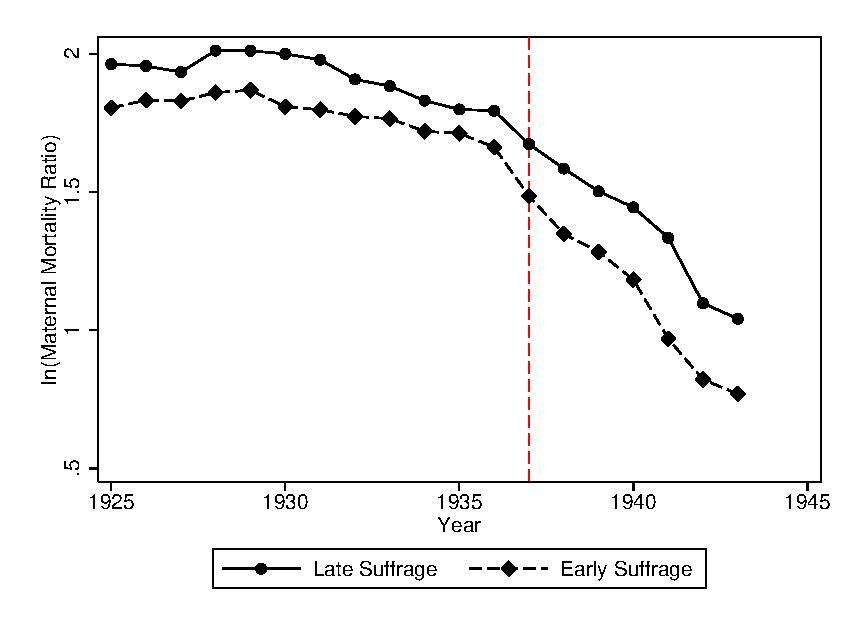
\includegraphics[scale=0.67]{./figures/MMRtrends.eps}
\end{figure}
{\footnotesize \hyperlink{USA}{\textcolor{blue}{back}}}
\end{frame}

\begin{frame}[plain,label=ptrends]
\begin{figure}[h!]
\centering
\caption{Trends in ln(IPR)}
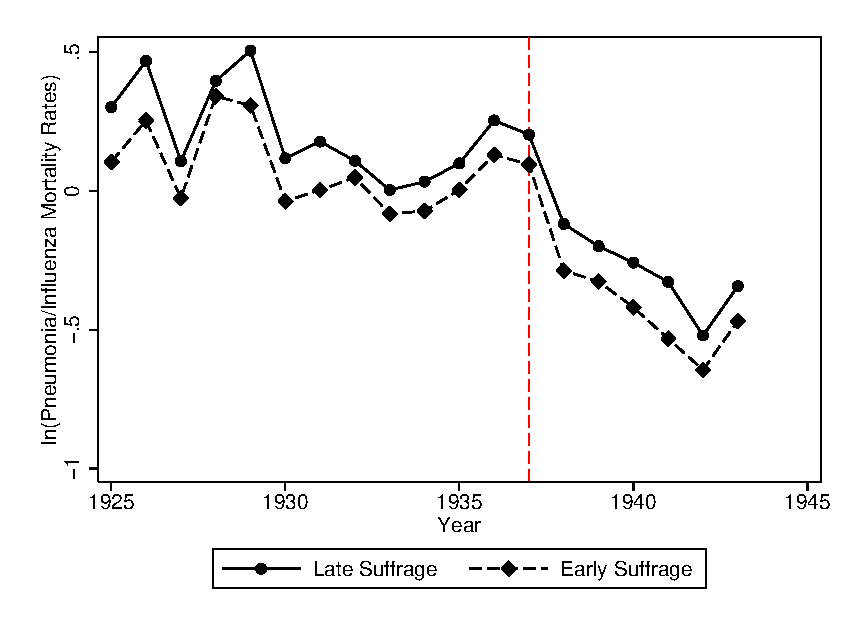
\includegraphics[scale=0.67]{./figures/IPRtrends.eps}
\end{figure}
{\footnotesize \hyperlink{USA}{\textcolor{blue}{back}}}
\end{frame}

\begin{frame}[plain,label=DDreg]
\begin{table}[htpb]
\begin{center}
\caption{Early Suffrage Adopters and Disease Burden}
\label{tab:sulfaSuffrage}
\scalebox{0.7}{
\begin{tabular}{lcc} \toprule
& 	(1) &	(2) \\
& log(MMR) & log(Pneumonia) \\ \midrule
		
Post-1937 &	-0.0917$^{***}$ &	0.00870 \\
&\begin{footnotesize}(0.0298)\end{footnotesize}	&\begin{footnotesize}(0.0215)\end{footnotesize} \\
Post$\times$Year&	-0.0891$^{***}$ &	-0.0611$^{***}$ \\
&\begin{footnotesize}	(0.00490)\end{footnotesize}	&\begin{footnotesize}	(0.0108)\end{footnotesize} \\
Year&	-0.0230$^{***}$&	-0.0293$^{***}$ \\
&\begin{footnotesize}	(0.00246)	\end{footnotesize}	&\begin{footnotesize}(0.00647)\end{footnotesize} \\
Early Suffrage $\times$ Post &	-0.0849$^{**}$ &	-0.0459 \\
&\begin{footnotesize}	(0.0365)\end{footnotesize}	&\begin{footnotesize}	(0.0279)\end{footnotesize} \\
Early Suffrage $\times$ Post $\times$ Year	&-0.0146$^{**}$ &	-0.00674 \\
&\begin{footnotesize}	(0.00642)\end{footnotesize}	&\begin{footnotesize}	(0.0128)\end{footnotesize} \\
Early Suffrage $\times$ Year&	0.001000 &	0.00470 \\
&\begin{footnotesize}	(0.00335)\end{footnotesize}	&\begin{footnotesize}	(0.00760)\end{footnotesize} \\
Constant &	1.689$^{***}$	&-0.0461$^{***}$ \\
&\begin{footnotesize}	(0.0120)\end{footnotesize}	&\begin{footnotesize}	(0.0148)\end{footnotesize} \\ \midrule
Observations &	868	 & 868 \\
R-squared &	0.951 &	0.780 \\ \bottomrule
\end{tabular}}
\end{center}
\end{table}

{\footnotesize \hyperlink{USA}{\textcolor{blue}{back}}}
\end{frame}

\begin{frame}[label=WhySuffrage]
\frametitle{Why differences in Suffrage across states?}
\vspace{4mm}
\textit{``The most obvious pattern is geographic – all else equal, women in western states could vote before women elsewhere in America. Some historians suggest that frontier conditions were amenable to women's suffrage because women supported restrictions on common western vices (drunkenness, gambling, and prostitution) or because the harsh realities of frontier life made it impossible to maintain traditional gender roles (Brown 1958; Grimes 1967). Many others argue that idiosyncratic circumstances in each state resulted in the vote for women (Larson 1971; Beeton 1986), citing rich historical evidence in support of this view. Quantitative studies yield strikingly inconclusive results (Cornwall, Dahlin, King, and Schiffman 2004). \textbf{The single robust correlate of suffrage law enactment emerging from these studies is the share of women working in non-agricultural occupations} (King, Cornwall, and Dahlin 2005). Although this presumably reflects changing social norms about the role of women, it evolved very gradually over time (Smith and Ward 1985; Goldin 1990) and can be distinguished econometrically from abrupt year-to-year legislative changes governing women’s right to vote." \hyperlink{USAHistory}{\textcolor{blue}{Miller (2008)}}}\\
 \end{frame} 


%********************************************************************************
%********************************************************************************
%*** APPENDICES [Quotas]
%********************************************************************************
%********************************************************************************
\begin{frame}[plain]
\begin{center}
\textbf{Appendix II - Quotas}
\end{center}
\end{frame}
\begin{frame}
\frametitle{(2) Quotas and Women in Parliament}
The site \url{www.quotaproject.org} provides the most definitive source of
gender quotas in parliament at a national and sub-national level. \vspace{5mm}
\begin{itemize}
\setlength{\itemsep}{10pt}
\item We compiled data for each country recording whether or
  not reserved seats are legislated for women leaders
\item If so, we record the date the legislation was adopted
\item We also record the size of the quota (eg the percent of seats reserved for
  women)
\item The results here do \emph{not} include quotas at a sub-national level.
\end{itemize}
\end{frame}

\begin{frame}[label=quotaDesc]
  \begin{figure}
    \caption{Implementation of Reserved Seats for Women Leaders}
    \includegraphics[scale=0.5]{./figures/quotasStackedRes.eps}
  \end{figure}
\end{frame}


\begin{frame}[label=Quotas]
\frametitle{Quotas: Estimation and results}
We begin by estimating a diff-in-diff model of quota implementation:
\begin{equation}
  \label{quotareg}
\log(MMR)_{ct} = \alpha_0 + \alpha_1 Quota_{c,t-1} + \mu_c + \lambda_t + \varepsilon_{ct}  
\end{equation}
\vspace{4mm}
\begin{itemize}
\item Baseline specification includes country and year fixed effects
\item Standard errors clustered at level of country
\item Also include time-varying controls such as $\log(GDP pc)$
\item The direct effect of reserved seats on women in parliament is important
  \begin{itemize}
    \item Some countries are \hyperlink{quotaCover}{{\textcolor{blue}{particularly noteworthy} (Algeria, Burundi,\ldots)}} 
  \item Examine formally by estimating (\ref{quotareg}) with \% of women in parliament as outcome variable
  \end{itemize}
  \end{itemize}
\end{frame}

\begin{frame}[label=Quotas2]
\frametitle{Quotas: Estimation and results}
We then estimate a full event-study surrouding implementation:
\begin{eqnarray}
  \log(MMR)_{ct} &=& \alpha_0 + \sum_{j=1}^J \tau_{-j}\cdot Quota_{c,t-j} + \sum_{k=1}^K \tau_{+k}\cdot Quota_{c,t+k} \nonumber \\
  && + \mu_c + \lambda_t + \varepsilon_{ct} \nonumber
\end{eqnarray}
\begin{itemize}
\item We interact quota implementation with a full set of leads and lags
\item In the spirit of Granger (1969) casuality, we should observe that if any effects from (1) are truly due to quotas, these should emerge only after the reform, and not in the pre-reform coefficients $\tau_{-j}.$
\end{itemize}
\end{frame}

\begin{frame}[label=quotaCover]
  \begin{figure}
    \caption{Countries with Reserved Seats and Women's Representation}
    \includegraphics[scale=0.74]{./figures/ReservedCountries.eps}
  \end{figure}
  \hyperlink{Quotas}{{\footnotesize \textcolor{blue}{Back}}}
\end{frame}

\begin{frame}[label=quotalnMMR]
  \begin{figure}
    \caption{Event Study: Reserved Seats and Maternal Mortality Ratio}
    \includegraphics[scale=0.74]{./figures/eventMMRreserved.eps}
  \end{figure}
  \hyperlink{quotaMMR}{{\footnotesize \textcolor{blue}{Back}}}
\end{frame}



%********************************************************************************
%********************************************************************************
%*** APPENDICES [Worldwide]
%********************************************************************************
%********************************************************************************
\begin{frame}[plain]
\begin{center}
\textbf{Appendix III - Contemporary Cross-Country Gender Bias}
\end{center}
\end{frame}

\begin{frame}[label=CC]
\frametitle{Conditional Analysis}
We estimate the following regression using panel data:
	\begin{equation}
		MMR_{it} = \alpha + \beta GenderBias_{it} + \gamma_i + \delta_t + 
               (\phi_i\times t) + \theta X_{it} + \varepsilon_{it}. \nonumber
	\end{equation}
\vspace{4mm}
    \begin{itemize}
\setlength{\itemsep}{8pt}
	\item MMR is later replaced with the log ratio of female-male life expectancy.
  \item $GenderBias_{it}$ is measured as desired sex ratio of births, women's 
        rights and women's share of parliamentary seats.
	\item $\gamma$, $\delta$, $(\phi_i\times t)$ - country and year specific FE,
        country specific trends.  
  \item $X_{it}$ includes ln(GDP), interactions
	\item Standard errors are always clustered at the country level.
  \item We construct/collect data from various
        sources: \hyperlink{sumstatsWorld}{\textcolor{blue}{WB, WHO, DHS}}
\end{itemize}
\end{frame}



\begin{frame}[label=sumstatsWorld]
\frametitle{Cross country data sources}
\begin{table}[htbp]
\caption{Annual data  (with gaps)}
\scalebox{0.74}{
\begin{tabular}{lccc}
  \toprule
  Variable &     Source & N Countries &      Years \\
\midrule
MMR (Deaths per 100,000 live births) &        WDI &        183 & 1990- 2015 \\

Subnational MMR calculated from microdata &        DHS &         45 &  1970-2010 \\

Life Expectancy (Male) &        WDI &        200 &  1960-2014 \\

Life Expectancy (Female) &        WDI &        200 &  1960-2015 \\

Life Expectancy Ratio (F/M) &        WDI &        200 &  1960-2016 \\

       GDP &        WDI &        190 &  1960-2015 \\

Tuberculosis Mortality Rate &        WDI &        191 &  1990-2015 \\

Desired Sex Ratio (M/F) &        DHS &         63 &  1960-2012 \\

Women's Political Rights &  Cingareli &        190 &  1981-2011 \\

Women's Economic Rights &  Cingareli &        190 &  1981-2011 \\

Women's Social Rights &  Cingareli &        190 &  1981-2004 \\
\bottomrule
\end{tabular}}  
\end{table}
\hyperlink{CC}{\textcolor{blue}{Back}}
\end{frame}


\begin{frame}
\begin{table}[htbp]\centering 
\caption{Summary statistics \label{sumstat}}
\scalebox{0.74}{
  \begin{tabular}{l c c c c c}
    \toprule
\multicolumn{1}{c}{\textbf{Variable}} & \textbf{Mean}
 & \textbf{Std. Dev.}& \textbf{Min.} &  \textbf{Max.} & \textbf{N}\\ 
\midrule
Life Expectancy (Female)& 65.709 & 12.176 & 22.394 & 86.900 & 10629\\
Life Expectancy (Male) & 61.106 & 10.925 & 16.286 & 81.600 & 10629\\
LE ratio (F/M) & 1.074 & 0.036 & 0.963 & 1.375 & 10629\\
MMR & 251.57 & 357.733 & 3 & 2900 & 4758\\
Log GDP & 8.201 & 1.509 & 4.749 & 11.886 & 8342\\
Desired Sex Ratio (M/F) & 1.116 & 0.142 & 0.433 & 3 & 2997\\
Tuberculosis Mortality Rate & 21.559 & 32.145 & 0 & 283 & 4712\\
Women's Political Rights & 1.786 & 0.647 & 0 & 3 & 4830\\
Women's Economic Rights  & 1.323 & 0.697 & 0 & 3 & 4779\\
Women's Social Rights  & 1.235 & 0.84 & 0 & 3 & 3395\\
Women's Composite Rights 1& 0 & 1.436 & -3.435 & 3.882 & 3352\\
Women's Composite Rights 2 & 0 & 1.16 & -3.286 & 3.022 & 4766\\
%ngii grammar index& 0.46 & 0.498 & 0 & 1 & 6944\\
%sbii grammar index& 0.694 & 0.461 & 0 & 1 & 6944\\
%gaii grammar index& 0.692 & 0.462 & 0 & 1 & 5096\\
%gpii grammar index& 0.341 & 0.474 & 0 & 1 & 6888\\
%gt\_pronoun grammar index& 2.524 & 1.5 & 0 & 4 & 4592\\
%gii0 grammar index& 2.453 & 1.661 & 0 & 4 & 4816\\
%gii1 grammar index& 1.978 & 1.222 & 0 & 3 & 5096\\
%gii2 grammar index& 1.517 & 1.235 & 0 & 3 & 6496\\
\bottomrule
\end{tabular}}
\end{table}
\hyperlink{CC}{\textcolor{blue}{Back}}
\end{frame}


\begin{frame}[label=RightsComp]
\frametitle{Gender Bias Measured by Women's Composite Rights}
\begin{table}[htbp]\centering
\caption{Maternal Mortality and Women's Composite Rights \label{MMRWRight3}}
\scalebox{0.7}{
\begin{tabular}{l*{6}{c}}
\hline\hline
            &\multicolumn{1}{c}{(1)}&\multicolumn{1}{c}{(2)}&\multicolumn{1}{c}{(3)}&\multicolumn{1}{c}{(4)}&\multicolumn{1}{c}{(5)}&\multicolumn{1}{c}{(6)}\\
            %&\multicolumn{1}{c}{indep0}&\multicolumn{1}{c}{indep1}&\multicolumn{1}{c}{indep2}&\multicolumn{1}{c}{indep3}&\multicolumn{1}{c}{indep4}&\multicolumn{1}{c}{indep5}\\
\hline
\multicolumn{1}{p{2cm}}{Political,Economic, }       &      -4.276         &      -3.094         &      -4.187         &      -122.3$^{***}$&      -126.0$^{***}$&      -115.4$^{***}$\\
  Social Rights          &     (4.518)         &     (4.662)         &     (4.827)         &     (32.68)         &     (33.64)         &     (31.59)         \\

log GDP        &      -101.7$^{***}$&      -37.54         &      -42.46         &      -32.60         &      -36.96         &      -70.65$^{*}$  \\
            &     (20.04)         &     (36.27)         &     (36.59)         &     (35.10)         &     (35.10)         &     (39.69)         \\

%democ       &                     &                     &      -2.130         &                     &      -1.713         &      -51.66$^{**}$ \\
%            &                     &                     &     (2.340)         &                     &     (2.306)         &     (19.83)         \\

Rights*log GDP    &                     &                     &                     &       14.84$^{***}$&       15.14$^{***}$&       13.80$^{***}$\\
            &                     &                     &                     &     (3.694)         &     (3.796)         &     (3.540)         \\

%Democracy * log GDP   &                     &                     &                     &                     &                     &       7.009$^{***}$\\
%            &                     &                     &                     &                     &                     &     (2.589)         \\

%\_cons      &      1143.2$^{***}$&       628.8$^{**}$ &       675.4$^{**}$ &       576.7$^{**}$ &       615.7$^{**}$ &       831.0$^{***}$\\
%            &     (172.3)         &     (293.8)         &     (297.1)         &     (283.7)         &     (284.6)         &     (310.6)         \\
\hline
\(N\)       &        2111         &        2111         &        1972         &        2111         &        1972         &        1972         \\
r2          &                     &       0.215         &       0.215         &       0.265         &       0.269         &       0.299         \\
\hline\hline

\multicolumn{1}{p{2cm}}{Political \& }       &      -3.590         &      -2.147         &      -3.371         &      -184.8$^{***}$&      -183.0$^{***}$&      -160.6$^{***}$\\
 Economic Rights          &     (5.952)         &     (6.161)         &     (6.956)         &     (43.70)         &     (47.74)         &     (43.13)         \\

log GDP        &      -96.69$^{***}$&      -37.17         &      -27.16         &      -22.23         &      -12.95         &      -63.28$^{*}$  \\
            &     (17.87)         &     (33.78)         &     (34.56)         &     (31.40)         &     (32.30)         &     (35.64)         \\

%democ       &                     &                     &      -7.795$^{*}$  &                     &      -6.608$^{*}$  &      -79.60$^{***}$\\
            &                     &                     &     (4.274)         &                     &     (3.914)         &     (25.41)         \\

Rights*log GDP    &                     &                     &                     &       22.28$^{***}$&       21.98$^{***}$&       19.29$^{***}$\\
            &                     &                     &                     &     (4.843)         &     (5.237)         &     (4.693)         \\

%Democracy * lgdp   &                     &                     &                     &                     &                     &       10.04$^{***}$\\
 %           &                     &                     &                     &                     &                     &     (3.113)         \\

%\_cons      &      1103.0$^{***}$&       621.9$^{**}$ &       578.0$^{**}$ &       489.0$^{*}$  &       444.8$^{*}$  &       776.0$^{***}$\\
%            &     (156.0)         &     (274.9)         &     (278.7)         &     (254.8)         &     (258.9)         &     (282.0)         \\
\hline
\(N\)       &        3400         &        3400         &        3113         &        3400         &        3113         &        3113         \\
r2          &                     &       0.245         &       0.263         &       0.313         &       0.327         &       0.369         \\
\hline
Country FE        &                     &    Y                 &      Y               &     Y         &           Y          &     Y         \\
Year FE            &                     &    Y                 &      Y               &     Y         &           Y          &     Y         \\
Democracy       &                     &                     &     Y &                     &      Y  &      Y\\
Democracy*log GDP   &                     &                     &                     &                     &                     &      Y\\

\hline
%\multicolumn{7}{l}{\footnotesize Standard errors in parentheses}\\
%\multicolumn{7}{l}{\footnotesize $^{*}$ \(p<0.10\), $^{**}$ \(p<0.05\), $^{***}$ \(p<0.01\)}\\
\end{tabular}}
\end{table}
\hyperlink{Rights}{\textcolor{blue}{Back}}
\end{frame}

\begin{frame}[plain]
\begin{center}
\textbf{Appendix IV - Historical Factors and Contemporary Outcomes}
\end{center}
\end{frame}

\begin{frame}[label=GenderLanguage]
\frametitle{Gender Bias and Grammatical Gender}
The literature has proposed a number of measures of gender intensity of language.
We follow recent papers in defining the following (summary statistics \hyperlink{GenderLanguageSum}{\textcolor{blue}{here}}): \vspace{4mm}
\begin{enumerate}
\item Sex-Based Intensity Index (sbii) 
\item Number Gender Intensity Index (ngii)
\item Gender Assignment Intensity Index (gaii) 
\item Gender Pronouns Intensity Index (gpii) 
\item gii0 = ngii + sbii + gaii + gpii
\item gii1 = ngii + sbii + gaii
\item gii2 = ngii + sbii + gpii
\item gtroiano = number of cases of gender differentiated pronouns.
\end{enumerate}
\end{frame}

\begin{frame}[label=GenderLanguageSum]
\frametitle{Summary Statistics (Gender Intensity of Language)}
  \begin{table}[htbp]\centering 
\caption{Summary statistics \label{sumstat}}
\scalebox{0.7}{
\begin{tabular}{l c c c c c}\hline\hline
\multicolumn{1}{c}{\textbf{Variable}} & \textbf{Mean}
 & \textbf{Std. Dev.}& \textbf{Min.} &  \textbf{Max.} & \textbf{N}\\ 
\hline
Number Gender Intensity Index & 0.46 & 0.498 & 0 & 1 & 6944\\
Sex-Based Intensity Index& 0.694 & 0.461 & 0 & 1 & 6944\\
Gender Assignment Intensity Index& 0.692 & 0.462 & 0 & 1 & 5096\\
Gender Pronouns Intensity Index & 0.341 & 0.474 & 0 & 1 & 6888\\
gtroiano& 2.524 & 1.5 & 0 & 4 & 4592\\
gii0 & 2.453 & 1.661 & 0 & 4 & 4816\\
gii1 & 1.978 & 1.222 & 0 & 3 & 5096\\
gii2 & 1.517 & 1.235 & 0 & 3 & 6496\\
\hline
\end{tabular}}
\end{table}
\hyperlink{GenderLanguage}{\textcolor{blue}{Back}}
\end{frame}


\frame{
\frametitle{Gender Bias and Grammatical Gender}
The in-built structures of language have been demonstrated to have effects on present-day gender equality measures.  We estimate: \vspace{3mm}
\begin{equation}
MMR_{it} = \beta_0 + \beta_1 GII_i + \beta_2 PercentLang_i + X_{it} + X_i  + \nu_{it} \nonumber
\end{equation}
\vspace{3mm}
\begin{itemize}
\setlength{\itemsep}{15pt}
  \item GII is highly pre-determined but it does not vary over time. So we
        include continent FE rather than country FE.
	\item The idea is that grammatical gender reflects gender attitudes in society
	\begin{itemize}
		\item Maternity leave policy differences (Givati and Troiano, 2012).
		\item Female labour force and political participation (Gay et al. 2013).
	\end{itemize}
%\begin{enumerate}
%\item Sex-Based Intensity Index (sbii) 
%\item Number Gender Intensity Index (ngii)
%\item Gender Assignment Intensity Index (gaii) 
%\item Gender Pronouns Intensity Index (gpii) 
%\item gii0 = ngii + sbii + gaii + gpii
%\item gii1 = ngii + sbii + gaii
%\item gii2 = ngii + sbii + gpii
%\item gtroiano = number of cases of gender differentiated pronouns.
%\end{enumerate}
%%\item Example: gender differentiated personal pronouns: 
%%	\begin{itemize}
%%		\item English (``He", ``She")  
%%		\item Spanish (\textit{``El"}, \textit{``Ella"}; \textit{``Ellos"},
%%          \textit{``Ellas"};\textit{``Nosotros"}, \textit{``Nosotras"};
%%          \textit{``Vosotros"}, \textit{``Vosotras"})
%%	\end{itemize}
\end{itemize}
}


\begin{frame}[label=MMRcompare]
\begin{figure}[htpb!]
  \begin{center}
    \caption{Comparison of MMR values from WDI-generated and author-generated DHS microdata}
    \label{fig:time}
    \begin{subfigure}{.5\textwidth}
      \centering
      \includegraphics[scale=0.36]{./figures/MMRcomparison.eps}
      \caption{Estimates by Country and Year}
      \label{fig:seatsWP}
    \end{subfigure}%
    \begin{subfigure}{.5\textwidth}
      \centering
      \includegraphics[scale=0.36]{./figures/MMRcomparison_country.eps}
      \caption{Estimates by Country}
      \label{fig:WPMMR}
    \end{subfigure}
  \end{center}
  %\floatfoot{\textsc{Notes}: (Left-hand panel) Each point refers to one country by year observation of MMR as measured by the WDI imputed value and the value calculated from DHS microdata. The dotted line is a fitted univariate regression line between the two series. The correlation coefficient between the two measures if 0.7038. (Right-hand panel) Each point refers to average log(MMR) in a particular country between 1990 and 2010 using the full series of available WDI imputed values for MMR and the value calculated from DHS microdata. Each country is labeled using its ISO code. The dotted line is a fitted univariate regression line between the two series. The correlation coefficient between the two measures if 0.8582.}
\end{figure}
\hyperlink{MMRSub}{\textcolor{blue}{Back}}
\end{frame}



%********************************************************************************
\section{Placebo}
\begin{frame}[plain]
\begin{center}
\textbf{Appendix V - Gender Neutral Placebo Tests}
\end{center}
\end{frame}


\begin{frame}[label=placebos]
\frametitle{(5) Gender Neutral Placebo Tests}
\begin{itemize}
\setlength{\itemsep}{15pt}
  \item Tuberculosis is a ``gender neutral'' infectious disease
  \item Frequently occurring (around 9 million cases in 2013). Incidence ranges
        from less than 10 cases per 100,000 people, to greater than 1,000 per
        100,000 (ie a range very similar to MMR)
  \item We estimate the same set of specifications with the same measures of
        gender bias, replacing MMR with TB.
  \item Same tests replacing MMR with TB largely lead to null results:
  \begin{itemize}
    \item \hyperlink{placebo2}{\textcolor{blue}{Desired Sex Ratio}}
    \item \hyperlink{placebo1}{\textcolor{blue}{Women's Rights as gender
                                                inequality proxy}}
    \item \hyperlink{placebo3}{\textcolor{blue}{Gender inequality embedded in
                                                language}}
  \end{itemize}
\end{itemize}
\end{frame}


\begin{frame}[label=placebo1]
%\begin{table}[htbp]\centering
\def\sym#1{\ifmmode^{#1}\else\(^{#1}\)\fi}
\caption{TB and Women's Rights}
\scalebox{0.6}{
\begin{tabular}{l*{6}{c}}
\toprule
                    &\multicolumn{1}{c}{(1)}   &\multicolumn{1}{c}{(2)}   &\multicolumn{1}{c}{(3)}   &\multicolumn{1}{c}{(4)}   &\multicolumn{1}{c}{(5)}   &\multicolumn{1}{c}{(6)}   \\
                    &          TB   &          TB   &          TB   &          TB   &          TB   &          TB   \\
\midrule

 \textsc{Panel A: Political Rights}&&&&&\\ 
Political Rights    &        8.84   &        0.49   &        0.60   &      -24.28   &      -29.22   &      -29.48   \\
                    &      [9.77]   &      [9.14]   &      [9.11]   &     [52.31]   &     [50.76]   &     [49.67]   \\

R-squared           &        0.86   &        0.86   &        0.86   &        0.86   &        0.86   &        0.86   \\
Observations        &        3163   &        3163   &        3163   &        3163   &        3163   &        3163   \\

 &&&&&& \\
 \textsc{Panel B: Economic Rights}&&&&&\\ 

Economic Rights     &       -3.69   &       -5.74   &       -5.44   &       -9.79   &      -11.02   &      -10.61   \\
                    &      [9.97]   &     [10.17]   &     [10.20]   &     [34.29]   &     [33.87]   &     [32.83]   \\

R-squared           &        0.86   &        0.86   &        0.86   &        0.86   &        0.86   &        0.86   \\
Observations        &        3152   &        3152   &        3152   &        3152   &        3152   &        3152   \\

 \midrule Year FE&&Y&Y&Y&Y&Y\\ Democracy controls &&&Y&&Y&Y\\ 
Rights$\times$ GDP &&&&Y&Y&Y\\ Democracy$\times$ GDP &&&&&&Y\\ \bottomrule
\end{tabular}}\end{table}

\begin{table}[htbp]\centering
\scriptsize
\caption{Dependent Variable: TB mortality rate and Women's rights}
\begin{tabular}{l*{6}{c}}
\hline\hline
            &\multicolumn{1}{c}{(1)}&\multicolumn{1}{c}{(2)}&\multicolumn{1}{c}{(3)}&\multicolumn{1}{c}{(4)}&\multicolumn{1}{c}{(5)}&\multicolumn{1}{c}{(6)}\\
            %&\multicolumn{1}{c}{indep0}&\multicolumn{1}{c}{indep1}&\multicolumn{1}{c}{indep2}&\multicolumn{1}{c}{indep3}&\multicolumn{1}{c}{indep4}&\multicolumn{1}{c}{indep5}\\
\hline
Political rights       &      -0.912         &      -0.813         &      -1.063         &      -25.19$^{***}$&      -25.54$^{***}$&      -22.91$^{**}$ \\
            &     (1.017)         &     (1.030)         &     (1.155)         &     (7.838)         &     (9.015)         &     (9.070)         \\

log GDP        &      -9.891$^{***}$&      -7.312         &      -8.710         &      -12.17$^{*}$  &      -13.66$^{*}$  &      -16.30$^{**}$ \\
            &     (2.761)         &     (6.777)         &     (7.127)         &     (6.838)         &     (7.251)         &     (8.203)         \\

democ       &                     &                     &      -0.274         &                     &      -0.128         &      -4.907$^{*}$  \\
            &                     &                     &     (0.380)         &                     &     (0.384)         &     (2.710)         \\

Rights * LGDP  &                     &                     &                     &       3.011$^{***}$&       3.041$^{***}$&       2.746$^{***}$\\
            &                     &                     &                     &     (0.893)         &     (1.033)         &     (1.042)         \\

democracy * LGDP   &                     &                     &                     &                     &                     &       0.656$^{*}$  \\
            &                     &                     &                     &                     &                     &     (0.345)         \\

%\_cons      &       110.8$^{***}$&       89.88         &       103.4$^{*}$  &       128.9$^{**}$ &       142.2$^{**}$ &       158.2$^{**}$ \\
%            &     (24.13)         &     (55.70)         &     (59.21)         &     (56.66)         &     (60.53)         &     (66.06)         \\
\hline
\(N\)       &        3504         &        3504         &        3135         &        3504         &        3135         &        3135         \\
r2          &                     &       0.123         &       0.127         &       0.149         &       0.152         &       0.160         \\
\hline\hline
Economic rights       &       0.240         &       0.277         &      -0.282         &      -3.527         &      -5.154         &      -4.511         \\
            &     (1.411)         &     (1.517)         &     (1.695)         &     (8.038)         &     (8.653)         &     (8.381)         \\

log GDP        &      -9.722$^{***}$&      -6.860         &      -8.100         &      -7.213         &      -8.576         &      -12.39         \\
            &     (2.673)         &     (6.715)         &     (7.006)         &     (7.119)         &     (7.470)         &     (8.638)         \\

democ       &                     &                     &      -0.250         &                     &      -0.248         &      -6.099$^{**}$ \\
            &                     &                     &     (0.384)         &                     &     (0.386)         &     (2.783)         \\

Rights* log GDP   &                     &                     &                     &       0.454         &       0.583         &       0.489         \\
            &                     &                     &                     &     (0.795)         &     (0.851)         &     (0.816)         \\

democracy * LGDP   &                     &                     &                     &                     &                     &       0.807$^{**}$ \\
            &                     &                     &                     &                     &                     &     (0.357)         \\

%\_cons      &       107.8$^{***}$&       84.62         &       97.05         &       87.47         &       100.8         &       125.6$^{*}$  \\
%            &     (24.44)         &     (56.35)         &     (59.42)         &     (59.71)         &     (63.24)         &     (70.69)         \\
\hline
\(N\)       &        3492         &        3492         &        3124         &        3492         &        3124         &        3124         \\
r2          &                     &       0.125         &       0.128         &       0.125         &       0.129         &       0.143         \\
\hline\hline
\end{tabular}
\end{table}


{\footnotesize \hyperlink{placebos}{\textcolor{blue}{back}}}
\end{frame}






\begin{frame}[label=DSRIMR]
\frametitle{Desired Sex Ratio and Infant Mortality}
%\begin{table}[h!]\centering
\def\sym#1{\ifmmode^{#1}\else\(^{#1}\)\fi}
\caption{Infant mortality and DSR (boys/girls)  \label{FIMRdsr}}
\scalebox{0.62}{
\begin{tabular}{l*{6}{c}}
\toprule
            &\multicolumn{1}{c}{(1)}&\multicolumn{1}{c}{(2)}&\multicolumn{1}{c}{(3)}&\multicolumn{1}{c}{(4)}&\multicolumn{1}{c}{(5)}&\multicolumn{1}{c}{(6)}\\
            &\multicolumn{1}{c}{OLS}&\multicolumn{1}{c}{Probit}&\multicolumn{1}{c}{OLS}&\multicolumn{1}{c}{Probit}&\multicolumn{1}{c}{OLS}&\multicolumn{1}{c}{Probit}\\
\hline
Female       &      -1.153\sym{***}&     -0.0801\sym{***}&      -2.716\sym{***}&      -0.194\sym{***}&      -2.729\sym{***}&      -0.195\sym{***}\\
            &    (0.0928)         &   (0.00614)         &     (0.163)         &   (0.00894)         &     (0.163)         &   (0.00900)         \\

%age\_at\_birth&      -1.376\sym{***}&     -0.0842\sym{***}&      -1.377\sym{***}&     -0.0843\sym{***}&      -1.381\sym{***}&     -0.0845\sym{***}\\
%            &    (0.0790)         &   (0.00375)         &    (0.0789)         &   (0.00375)         &    (0.0785)         &   (0.00372)         \\

%age\_at\_birth2&      0.0235\sym{***}&     0.00143\sym{***}&      0.0234\sym{***}&     0.00143\sym{***}&      0.0234\sym{***}&     0.00142\sym{***}\\
%            &   (0.00136)         & (0.0000682)         &   (0.00135)         & (0.0000680)         &   (0.00134)         & (0.0000673)         \\

Desired Sex Ratio&      0.0125         &     0.00167         &      -0.551\sym{***}&     -0.0389\sym{***}&      -0.571\sym{***}&     -0.0400\sym{***}\\
            &     (0.103)         &   (0.00668)         &    (0.0997)         &   (0.00660)         &    (0.0971)         &   (0.00647)         \\

%education\_years&      -0.403\sym{***}&     -0.0338\sym{***}&      -0.400\sym{***}&     -0.0336\sym{***}&      -0.382\sym{***}&     -0.0325\sym{***}\\
%            &    (0.0249)         &   (0.00152)         &    (0.0248)         &   (0.00152)         &    (0.0257)         &   (0.00159)         \\

Desired Sex Ratio*Female&                     &                     &       1.362\sym{***}&      0.0976\sym{***}&       1.369\sym{***}&      0.0981\sym{***}\\
            &                     &                     &     (0.121)         &   (0.00704)         &     (0.121)         &   (0.00707)         \\

%Desired Fertility&                     &                     &                     &                     &       0.208\sym{***}&      0.0121\sym{***}\\
%            &                     &                     &                     &                     &    (0.0359)         &   (0.00222)         \\

%\_cons      &       111.2\sym{***}&       5.210         &       112.1\sym{***}&       5.273\sym{***}&       111.0\sym{***}&       5.209         \\
%            &     (0.918)         &         (.)         &     (0.966)         &     (0.237)         &     (0.996)         &         (.)         \\
\hline
Desired Fertility&     No         &         No         &     No         &     No         &     Yes         &         Yes         \\
\hline
\(N\)       &     4524542         &     4524521         &     4524542         &     4524521         &     4524542         &     4524521         \\
$R^{2}$  / pseudo $R^{2}$& 0.0216  &       0.040         & 0.0218             &       0.041         &     0.0220          &       0.041         \\
%r2          &      0.0216         &                     &      0.0218         &                     &      0.0220         &                     \\
\bottomrule
\end{tabular}}
\end{table}


\begin{table}[h!]\centering
\caption{Infant mortality and DSR (boys/girls) }
\scalebox{0.62}{
\begin{tabular}{l*{6}{c}}
\toprule
            &\multicolumn{1}{c}{(1)}&\multicolumn{1}{c}{(2)}&\multicolumn{1}{c}{(3)}&\multicolumn{1}{c}{(4)}&\multicolumn{1}{c}{(5)}&\multicolumn{1}{c}{(6)}\\
            &\multicolumn{1}{c}{OLS}&\multicolumn{1}{c}{Probit}&\multicolumn{1}{c}{OLS}&\multicolumn{1}{c}{Probit}&\multicolumn{1}{c}{OLS}&\multicolumn{1}{c}{Probit}\\
\hline
Female       &      -1.153$^{***}$&     -0.0801$^{***}$&      -2.716$^{***}$&      -0.194$^{***}$&      -2.729$^{***}$&      -0.195$^{***}$\\
            &    (0.0928)         &   (0.00614)         &     (0.163)         &   (0.00894)         &     (0.163)         &   (0.00900)         \\

%age\_at\_birth&      -1.376$^{***}$&     -0.0842$^{***}$&      -1.377$^{***}$&     -0.0843$^{***}$&      -1.381$^{***}$&     -0.0845$^{***}$\\
%            &    (0.0790)         &   (0.00375)         &    (0.0789)         &   (0.00375)         &    (0.0785)         &   (0.00372)         \\

%age\_at\_birth2&      0.0235$^{***}$&     0.00143$^{***}$&      0.0234$^{***}$&     0.00143$^{***}$&      0.0234$^{***}$&     0.00142$^{***}$\\
%            &   (0.00136)         & (0.0000682)         &   (0.00135)         & (0.0000680)         &   (0.00134)         & (0.0000673)         \\

Desired Sex Ratio&      0.0125         &     0.00167         &      -0.551$^{***}$&     -0.0389$^{***}$&      -0.571$^{***}$&     -0.0400$^{***}$\\
            &     (0.103)         &   (0.00668)         &    (0.0997)         &   (0.00660)         &    (0.0971)         &   (0.00647)         \\

%education\_years&      -0.403$^{***}$&     -0.0338$^{***}$&      -0.400$^{***}$&     -0.0336$^{***}$&      -0.382$^{***}$&     -0.0325$^{***}$\\
%            &    (0.0249)         &   (0.00152)         &    (0.0248)         &   (0.00152)         &    (0.0257)         &   (0.00159)         \\

Desired Sex Ratio*Female&                     &                     &       1.362$^{***}$&      0.0976$^{***}$&       1.369$^{***}$&      0.0981$^{***}$\\
            &                     &                     &     (0.121)         &   (0.00704)         &     (0.121)         &   (0.00707)         \\

%Desired Fertility&                     &                     &                     &                     &       0.208$^{***}$&      0.0121$^{***}$\\
%            &                     &                     &                     &                     &    (0.0359)         &   (0.00222)         \\

%\_cons      &       111.2$^{***}$&       5.210         &       112.1$^{***}$&       5.273$^{***}$&       111.0$^{***}$&       5.209         \\
%            &     (0.918)         &         (.)         &     (0.966)         &     (0.237)         &     (0.996)         &         (.)         \\
\hline
Desired Fertility&     No         &         No         &     No         &     No         &     Yes         &         Yes         \\
\hline
\(N\)       &     4524542         &     4524521         &     4524542         &     4524521         &     4524542         &     4524521         \\
$R^{2}$  / pseudo $R^{2}$& 0.0216  &       0.040         & 0.0218             &       0.041         &     0.0220          &       0.041         \\
%r2          &      0.0216         &                     &      0.0218         &                     &      0.0220         &                     \\
\bottomrule
\end{tabular}}
\end{table}
{\footnotesize \hyperlink{DSR}{\textcolor{blue}{back}}}
\end{frame}




%%DD moved some commented out parts down here so tex is easier to read. it would be good to see what was removed so when there's time good to un-comment this and let it be visible for us in appendix.


%\begin{frame}[label=CC2]
%\frametitle{Stylised Facts}
%\begin{figure}[htpb!]
%\centering
%\begin{subfigure}{.5\textwidth}
%  \centering
%  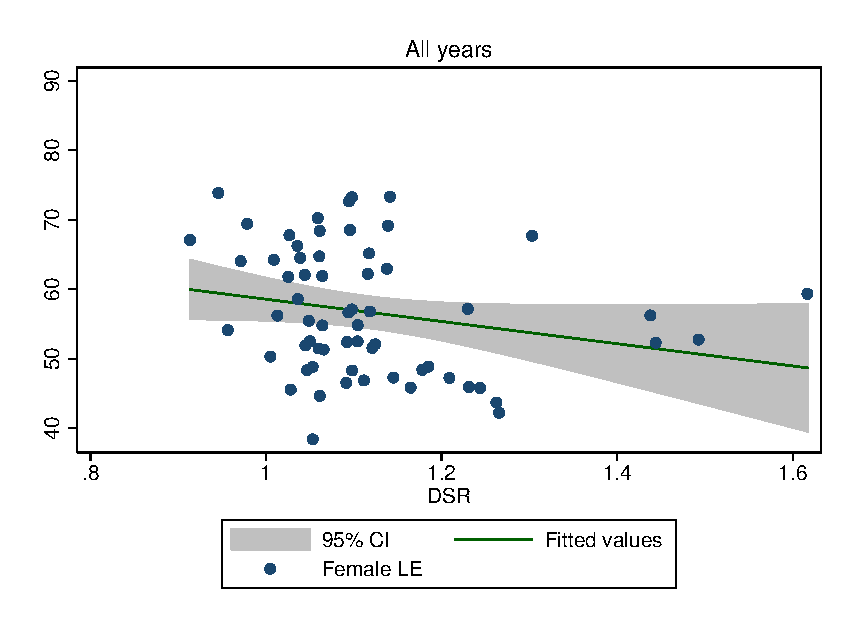
\includegraphics[scale=0.36]{./figures/lLEdesiredall.eps}
%  \caption{Female LE and DSR}
%  \label{TWINfig:fertrend}
%\end{subfigure}%
%\begin{subfigure}{.5\textwidth}
%  \centering
%  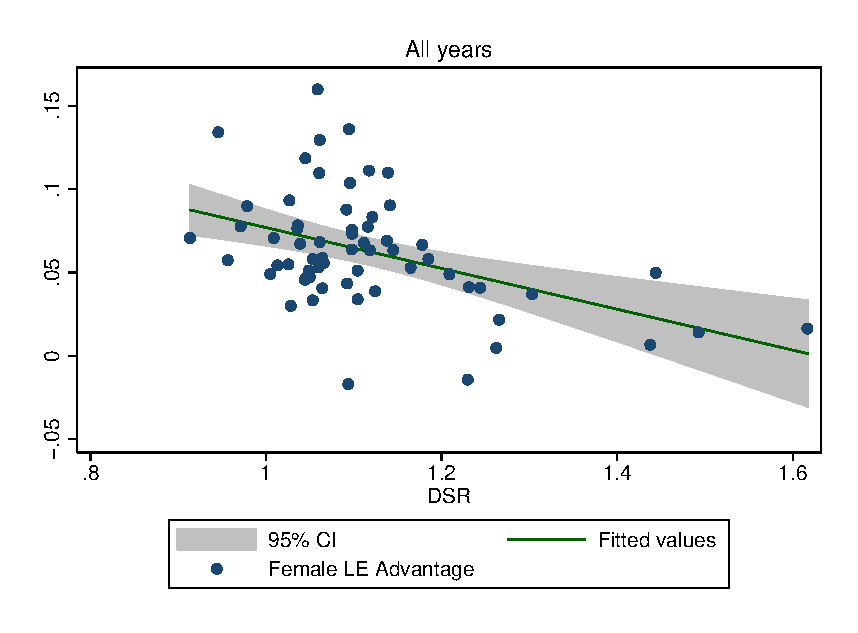
\includegraphics[scale=0.36]{./figures/lLErdesiredall.eps}
%  \caption{Female LE advantage and DSR}
%  \label{TWINfig:eductrend}
%\end{subfigure}
%\end{figure}
%\begin{itemize}
%\item The LE ratio is much more strongly related to gender bias
%\item Here gender bias is proxied by the desired sex ratio (desired number of boys to girls) reported by parents
%\item In other words, decreasing observable measures of gender bias \emph{does} improve gender equality in health outcomes
%\end{itemize}
%
%\end{frame}



%DCremove\frame{
%DCremove\frametitle{Wider Angle: Life Expectancy}
%DCremove\begin{itemize}
%DCremove\setlength{\itemsep}{20pt}
%DCremove	\item In early 20th century America, maternal mortality was the $2^{nd}$ largest cause of death for women of reproductive age, after TB (which affected men equally): Alabanesi \& Olivetti (2009). 
%DCremove		\vspace{3mm}
%DCremove		\begin{itemize}
%DCremove		\setlength{\itemsep}{12pt}
%DCremove		\item Similar magnitude in poor countries today although also CVD, injuries in India and HIV/AIDS in Africa.
%DCremove		\end{itemize}
%DCremove	\item MMR contributes to female life expectancy.
%DCremove	\vspace{3mm}
%DCremove		\begin{itemize}
%DCremove		\setlength{\itemsep}{12pt}
%DCremove		\item MMR declined by around 30\% in the late 1930s in America, raising the female-male LE differential at age 20 from 1.5 years in 1920 to 6 years in 1960. 
%DCremove		\item In the OECD the average female advantage in life expectancy during 1960-2011 was 6 years. 
%DCremove		\item In SS-Africa it is 2-3 years and in S-Asia it is close to zero.
%DCremove\end{itemize}
%DCremove\end{itemize}
%DCremove}

%DCremove\frame{
%DCremove\frametitle{MMR: Brazil vs. India - A contrast}
%DCremove	\begin{itemize}
%DCremove	\setlength{\itemsep}{20pt}
%DCremove		\item India: MMR was 390 in 100,000 and women's life expectancy advantage was 0.59 years in 2000. 
%DCremove		\item Contrast with Brazil: MMR of 84 and women had a LE advantage of 6.1 years.
%DCremove		\item Brazil adopted the Right to Health and implemented Universal Health Coverage and an emphasis on women's health ahead of other poor countries.
%DCremove	\end{itemize}
%DCremove}

%\frame{
%\frametitle{MMR and Excess female mortality}
%\begin{table}[htbp]\centering
%\footnotesize
%\def\sym#1{\ifmmode^{#1}\else\(^{#1}\)\fi}
%\caption{Mortality in the Reproductive ages (15-49)}
%\begin{tabular}{l*{3}{c}}
%\hline\hline
            %&\multicolumn{1}{c}{(1)}&\multicolumn{1}{c}{(2)}&\multicolumn{1}{c}{(3)}\\
            %&\multicolumn{1}{c}{Male}&\multicolumn{1}{c}{Female}&\multicolumn{1}{c}{Ratio (F/M)}\\
%\hline
%Log of MMR        & 0.0326         & 0.0767$^{**}$ & 0.0442$^{**}$ \\
            %&(0.0373)         &(0.0386)         &  (0.0181)         \\
%[1em]
%Log of GDP      & -0.0877$^{***}$& -0.111$^{***}$&  -0.0229         \\
            %& (0.0320)         & (0.0376)         & (0.0142)         \\
%\hline
%\(N\)       &               697 &         697         &  697         \\
%r2          &           0.0982   &       0.147         &  0.0678         \\
%\hline\hline
%\multicolumn{4}{l}{\footnotesize Standard errors in parentheses. }\\
%\multicolumn{4}{l}{\footnotesize All specifications have country and year FE.}\\
%\end{tabular}
%\end{table}
%}
%


%DCremove\frame{
%DCremove\frametitle{Hypothesis}
%DCremove\begin{itemize}
%DCremove\setlength{\itemsep}{20pt}
%DCremove		\item Mechansim?
%DCremove		\vspace{3mm}
%DCremove	\begin{itemize}
%DCremove	\setlength{\itemsep}{15pt}
%DCremove		\item Son preference - high \textit{fertility} - higher maternal mortality risk per woman (mechanical) and among higher order births (maternal depletion). E.g. Milazzo (2014).
%DCremove		\begin{itemize}
%DCremove		\vspace{1.5mm}
%DCremove			\item We investigate \textit{MMR per birth}
%DCremove		\end{itemize}
%DCremove		\item \textbf{Policy priorities} - resources to MMR (woman- specific) vs competing priorities: TB, infant diarrhea, pneumonia, measles, malaria. 
%DCremove		%\begin{itemize}
%DCremove			%\item Historical introduction of antibiotics in the US
%DCremove			%\item Reduced form approach with TB as a placebo disease
%DCremove			%\item Historical intra-country and cross-country gender prejudice determinants
%DCremove		%\end{itemize}
%DCremove	\end{itemize}
%DCremove\end{itemize}
%DCremove}

%  \begin{itemize}
%  \setlength{\itemsep}{7pt}
%\item In previous work, Bhalotra and Clarke (2013) show that exogenous increases in women's education created by program interventions are associated with large declines in MMR.
%\item We exploit variation in contemporary institutions giving women more voice and decision making power:
%  \begin{itemize}
%  \item The implementation of women's suffrage across the US states in the early 20th century  (Miller 2008).
%  \item Implementation of election quotas across countries since the 1990s (\url{www.quotaproject.org}).
%  \end{itemize}
%\item And historical given institutions/preferences:
%  \begin{itemize}
%  \item In language at birth on premise that gender differentiation embedded in language structure proxies deep-set (centuries old) gender attitudes (Gay et al. 2013). 
%  \item In elicited son preference in fertility
%  \item In institutionalized political, economic and social rights of women. 
%  \item Historical intra-country and cross-country gender prejudice determinants.
%  \end{itemize}
%\end{itemize}






%DCremove\subsection{Plough Use}
%DCremove\begin{frame}[label=PlowSlide]
%DCremove\frametitle{Plough use and reduction in maternal mortality}
%DCremove\begin{equation}
%DCremoveMMR_{it} = \beta_0 + \beta_1 plough_i + \beta_2 plough_i*lgdp_i + X_{it} + X_i  + \nu_{it} \nonumber
%DCremove\end{equation}
%DCremove\begin{itemize}
%DCremove\setlength{\itemsep}{15pt}
%DCremove  \item $plough_i$ comes from Alesina et al. (2013) indicating historical plough use in country $i$
%DCremove	\item Also highly pre-determined but it does not vary over time. 	So we
%DCremove        include continent FE rather than country FE.
%DCremove	\item However, in some specs we include country and year FE with only interaction of plough with either Log GDP or Women in Parliament.		
%DCremove	\item In the \hyperlink{PlowResults}{\textcolor{blue}{specs}}  using country and year FE, we find that both GDP and women in parliament have a smaller effect on MMR in societies which traditionally practiced plough agriculture. 	
%DCremove\end{itemize}
%DCremove\end{frame}
%DCremove
%DCremove
%DCremove
%DCremove\begin{frame}[label=PlowResults]
%DCremove\frametitle{Plough use and reduction in maternal mortality}
%DCremove\begin{table}[htbp]\centering
%DCremove\caption{MMR and plough use}
%DCremove\scalebox{0.8}{
%DCremove\begin{tabular}{l*{4}{c}}
%DCremove\hline\hline
%DCremove            &\multicolumn{1}{c}{(1)}&\multicolumn{1}{c}{(2)}&\multicolumn{1}{c}{(3)}&\multicolumn{1}{c}{(4)}\\
%DCremove            %&\multicolumn{1}{c}{est1}&\multicolumn{1}{c}{est2}&\multicolumn{1}{c}{est3}&\multicolumn{1}{c}{est4}&\multicolumn{1}{c}{est5}\\
%DCremove\hline
%DCremovePlough use        &      -173.9$^{***}$&      -28.32         &      -410.7$^{*}$  &                           \\
%DCremove            &     (62.75)         &     (44.07)         &     (221.1)         &                                    \\
%DCremove
%DCremoveLog GDP        &                     &      -99.47$^{***}$&      -133.2$^{***}$&      -195.6$^{***}$\\
%DCremove            &                     &     (19.87)         &     (24.22)         &     (34.37)               \\
%DCremove
%DCremovePlough $\times$ Log GDP   &                     &                     &       46.70$^{**}$ &       206.3$^{***}$               \\
%DCremove            &                     &                     &     (23.55)         &     (48.50)                         \\
%DCremove
%DCremove            &                     &                     &                     &                         \\
%DCremove\hline
%DCremove\(N\)       &        4654         &        3865         &        3865         &        4415               \\
%DCremover2          &       0.514         &       0.711         &       0.715         &       0.336                \\
%DCremove\hline\hline
%DCremove%\multicolumn{5}{l}{\footnotesize * \(p<0.10\), ** \(p<0.05\), *** \(p<0.01\)}\\
%DCremove\multicolumn{5}{p{10.2cm}}{\footnotesize The dependent variables is MMR (deaths per 100,000 births) from WDI. The first 3 columns use continent and decade fixed effects (but no country or year fixed effects) along with controls for log population; percentage of protestants, muslims and catholics; and proportion of country that's tropical. In the final column we use country and year fixed effects instead.}\\
%DCremove\end{tabular}}
%DCremove\end{table}
%DCremove %\hyperlink{PlowSlide}{\textcolor{blue}{Back}}  
%DCremove\end{frame}
\end{document}



